\chapter{実験結果}
% 第6章: 実験結果
% 本章では実験結果を客観的に報告する

本章では、第5章で述べた実験設定に基づき、96シナリオにおける4手法の性能評価結果を報告する。表\ref{tab:overall_summary}に全体統計サマリーを示す。

\begin{table}[htbp]
\centering
\caption{全体統計サマリー（96シナリオ）}
\label{tab:overall_summary}
\begin{tabular}{lccc}
\hline
手法 & 計算時間 [s] & 経路長 [m] & 成功率 [\%] \\
\hline
TA* & 15.46 & 21.27 & 96.88 \\
AHA* & 0.016 & 21.39 & 94.79 \\
Theta* & 0.234 & 23.64 & 100.00 \\
Field D* Hybrid & 0.175 & 23.60 & 100.00 \\
\hline
\end{tabular}
\end{table}

TA*は最短経路（21.27m）を達成したが、計算時間は平均15.46秒を要した。AHA*は最速（0.016秒）だが成功率94.79\%に留まった。Field D* Hybridは0.175秒で100\%の成功率を達成した。以下、各指標について詳細に分析する。

\section{経路長の比較}

第5章で述べた実験設定に基づき、各手法の経路長を比較した。図\ref{fig:path_length}に全96シナリオにおける各手法の平均経路長を示す。TA*が21.27mで最短経路を達成した。AHA*は21.39m、Field D* Hybridは23.60m、Theta*は23.64mであった。TA*とAHA*の差はわずか0.12m（0.56\%）であり、地形回避と最短経路を両立したことを示している。

\begin{figure}[htbp]
\centering
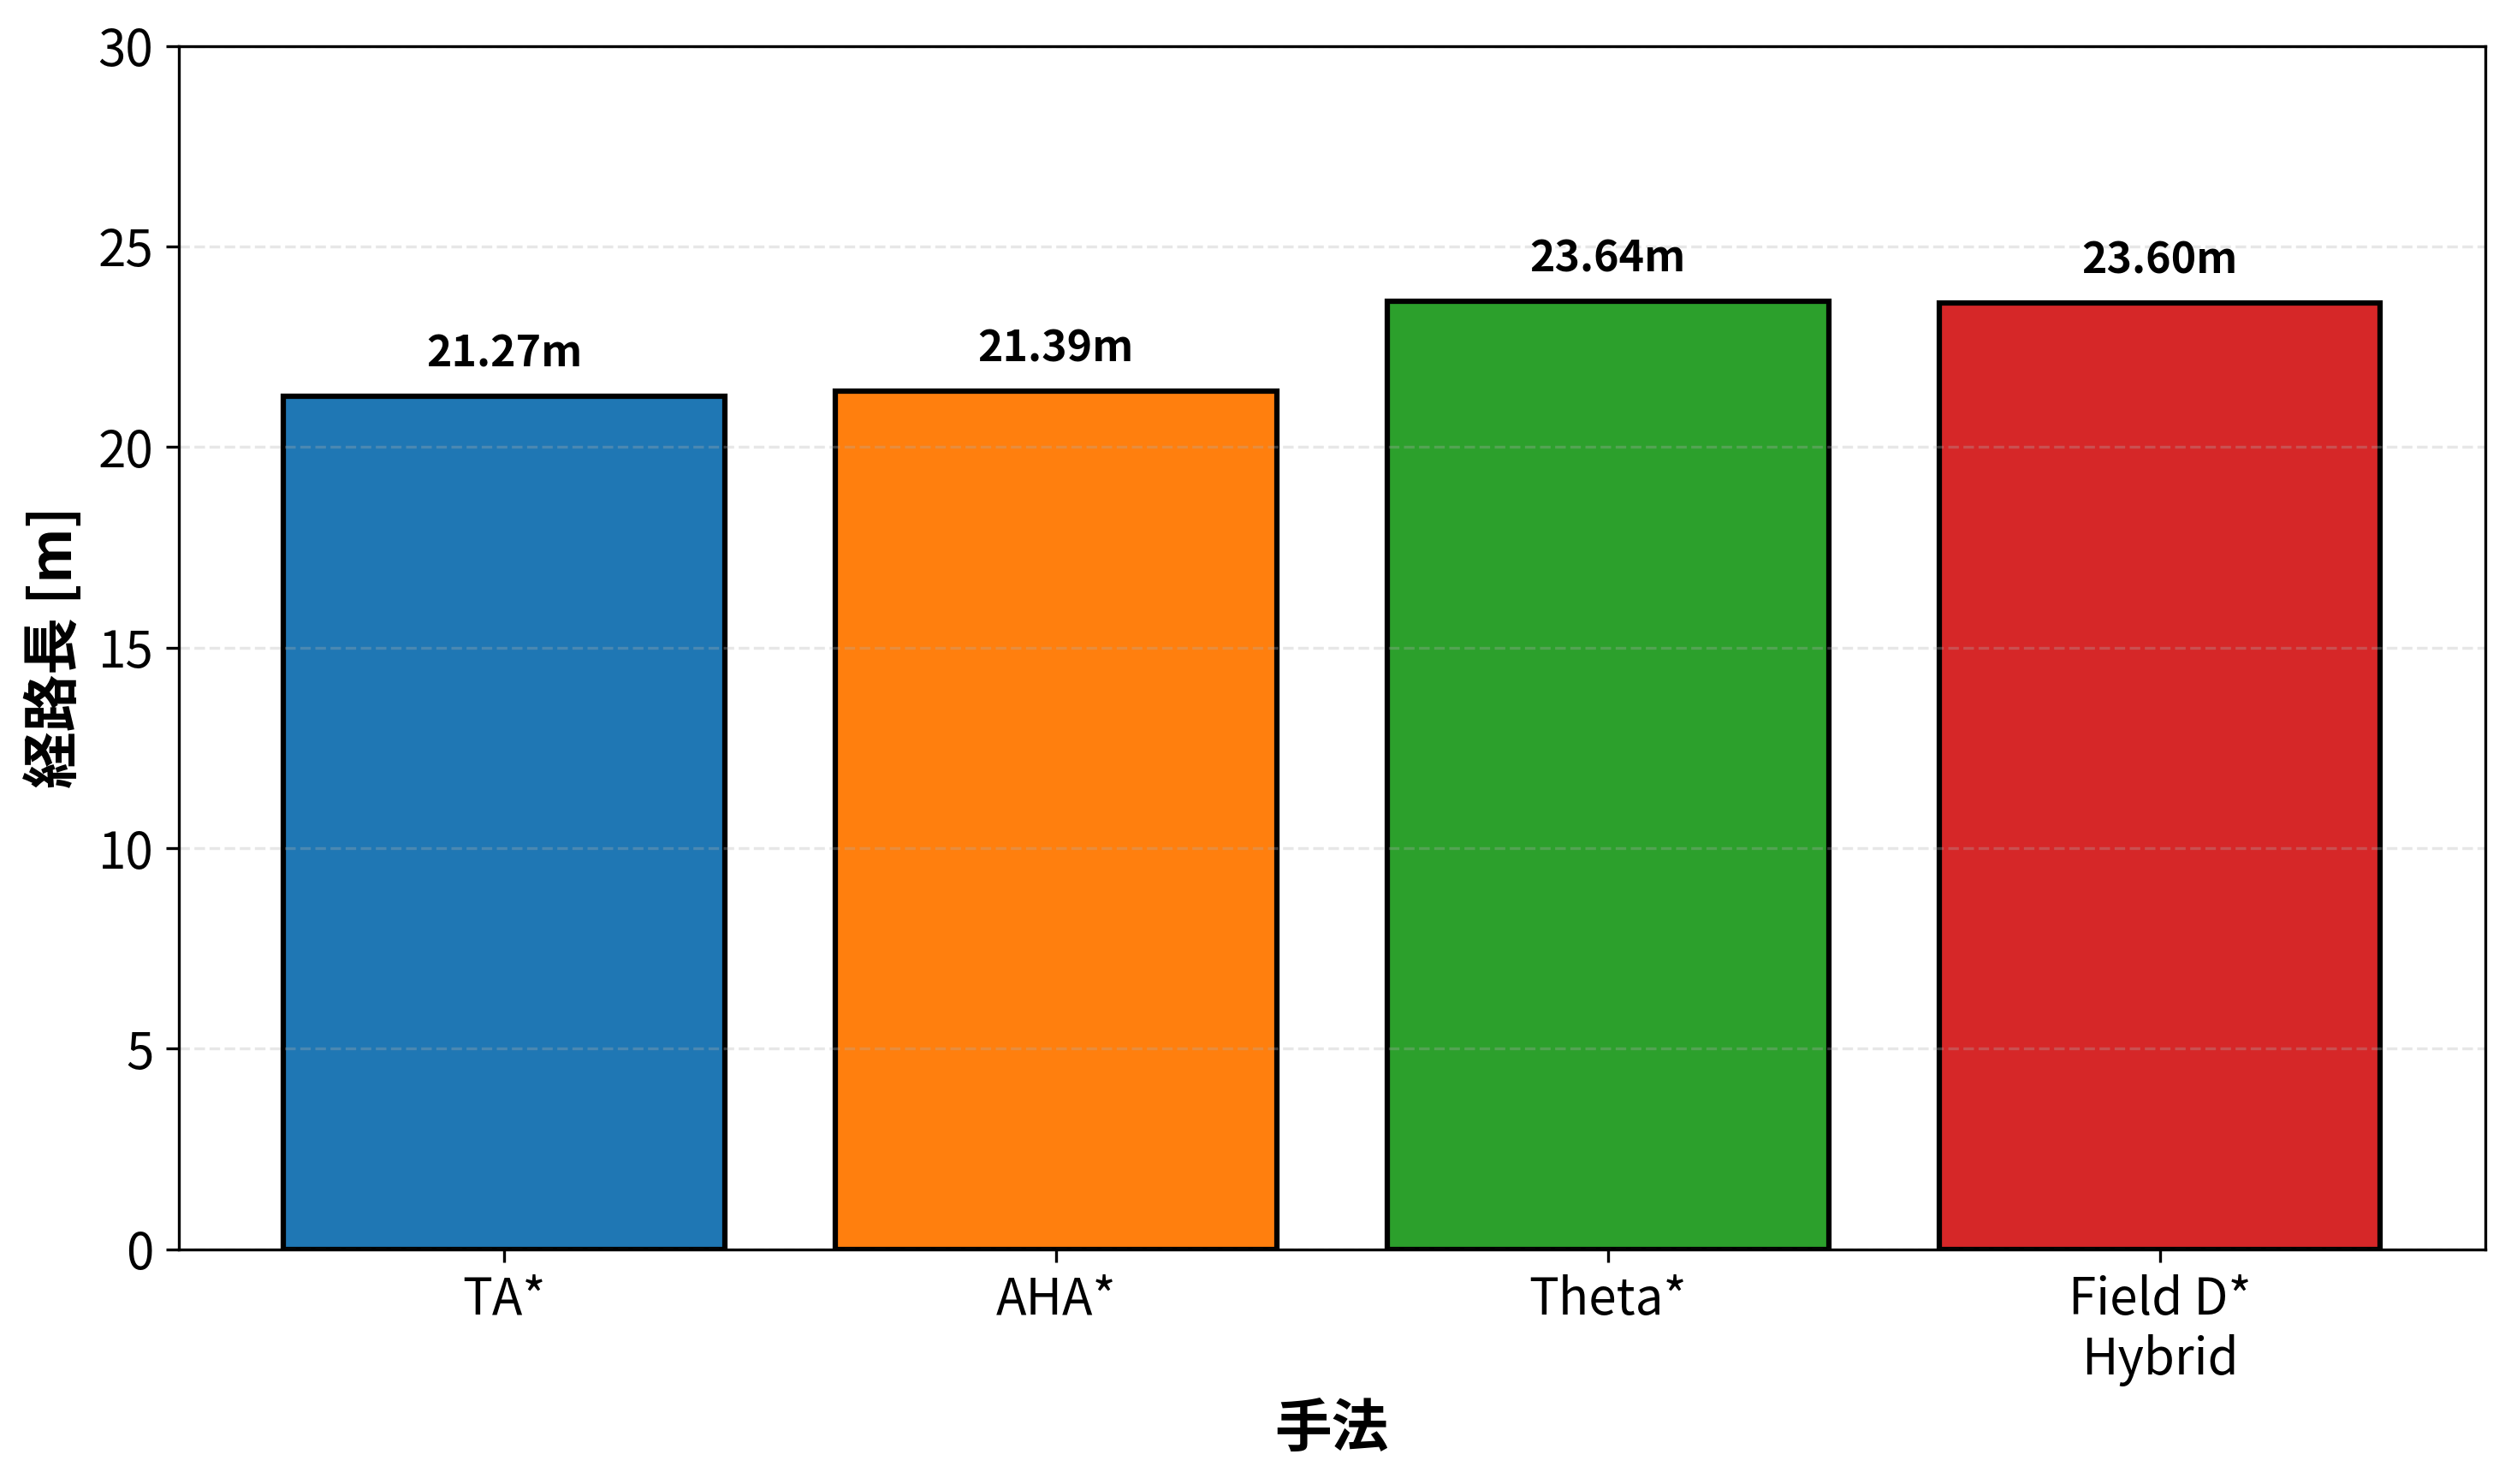
\includegraphics[width=0.9\textwidth,keepaspectratio]{figures/fig1_path_length.png}
\caption{全96シナリオにおける経路長比較}
\label{fig:path_length}
\end{figure}

\subsection{経路長の分布分析}

図\ref{fig:path_length_boxplot}に4手法の経路長の箱ひげ図を示す。全手法で多数の外れ値が見られるが、これらは地形変化が大きいシナリオや障害物が密に配置されたシナリオに対応している。TA*とAHA*の中央値はほぼ同一であり、両手法の経路長が同程度であることが確認できる。

\begin{figure}[htbp]
\centering
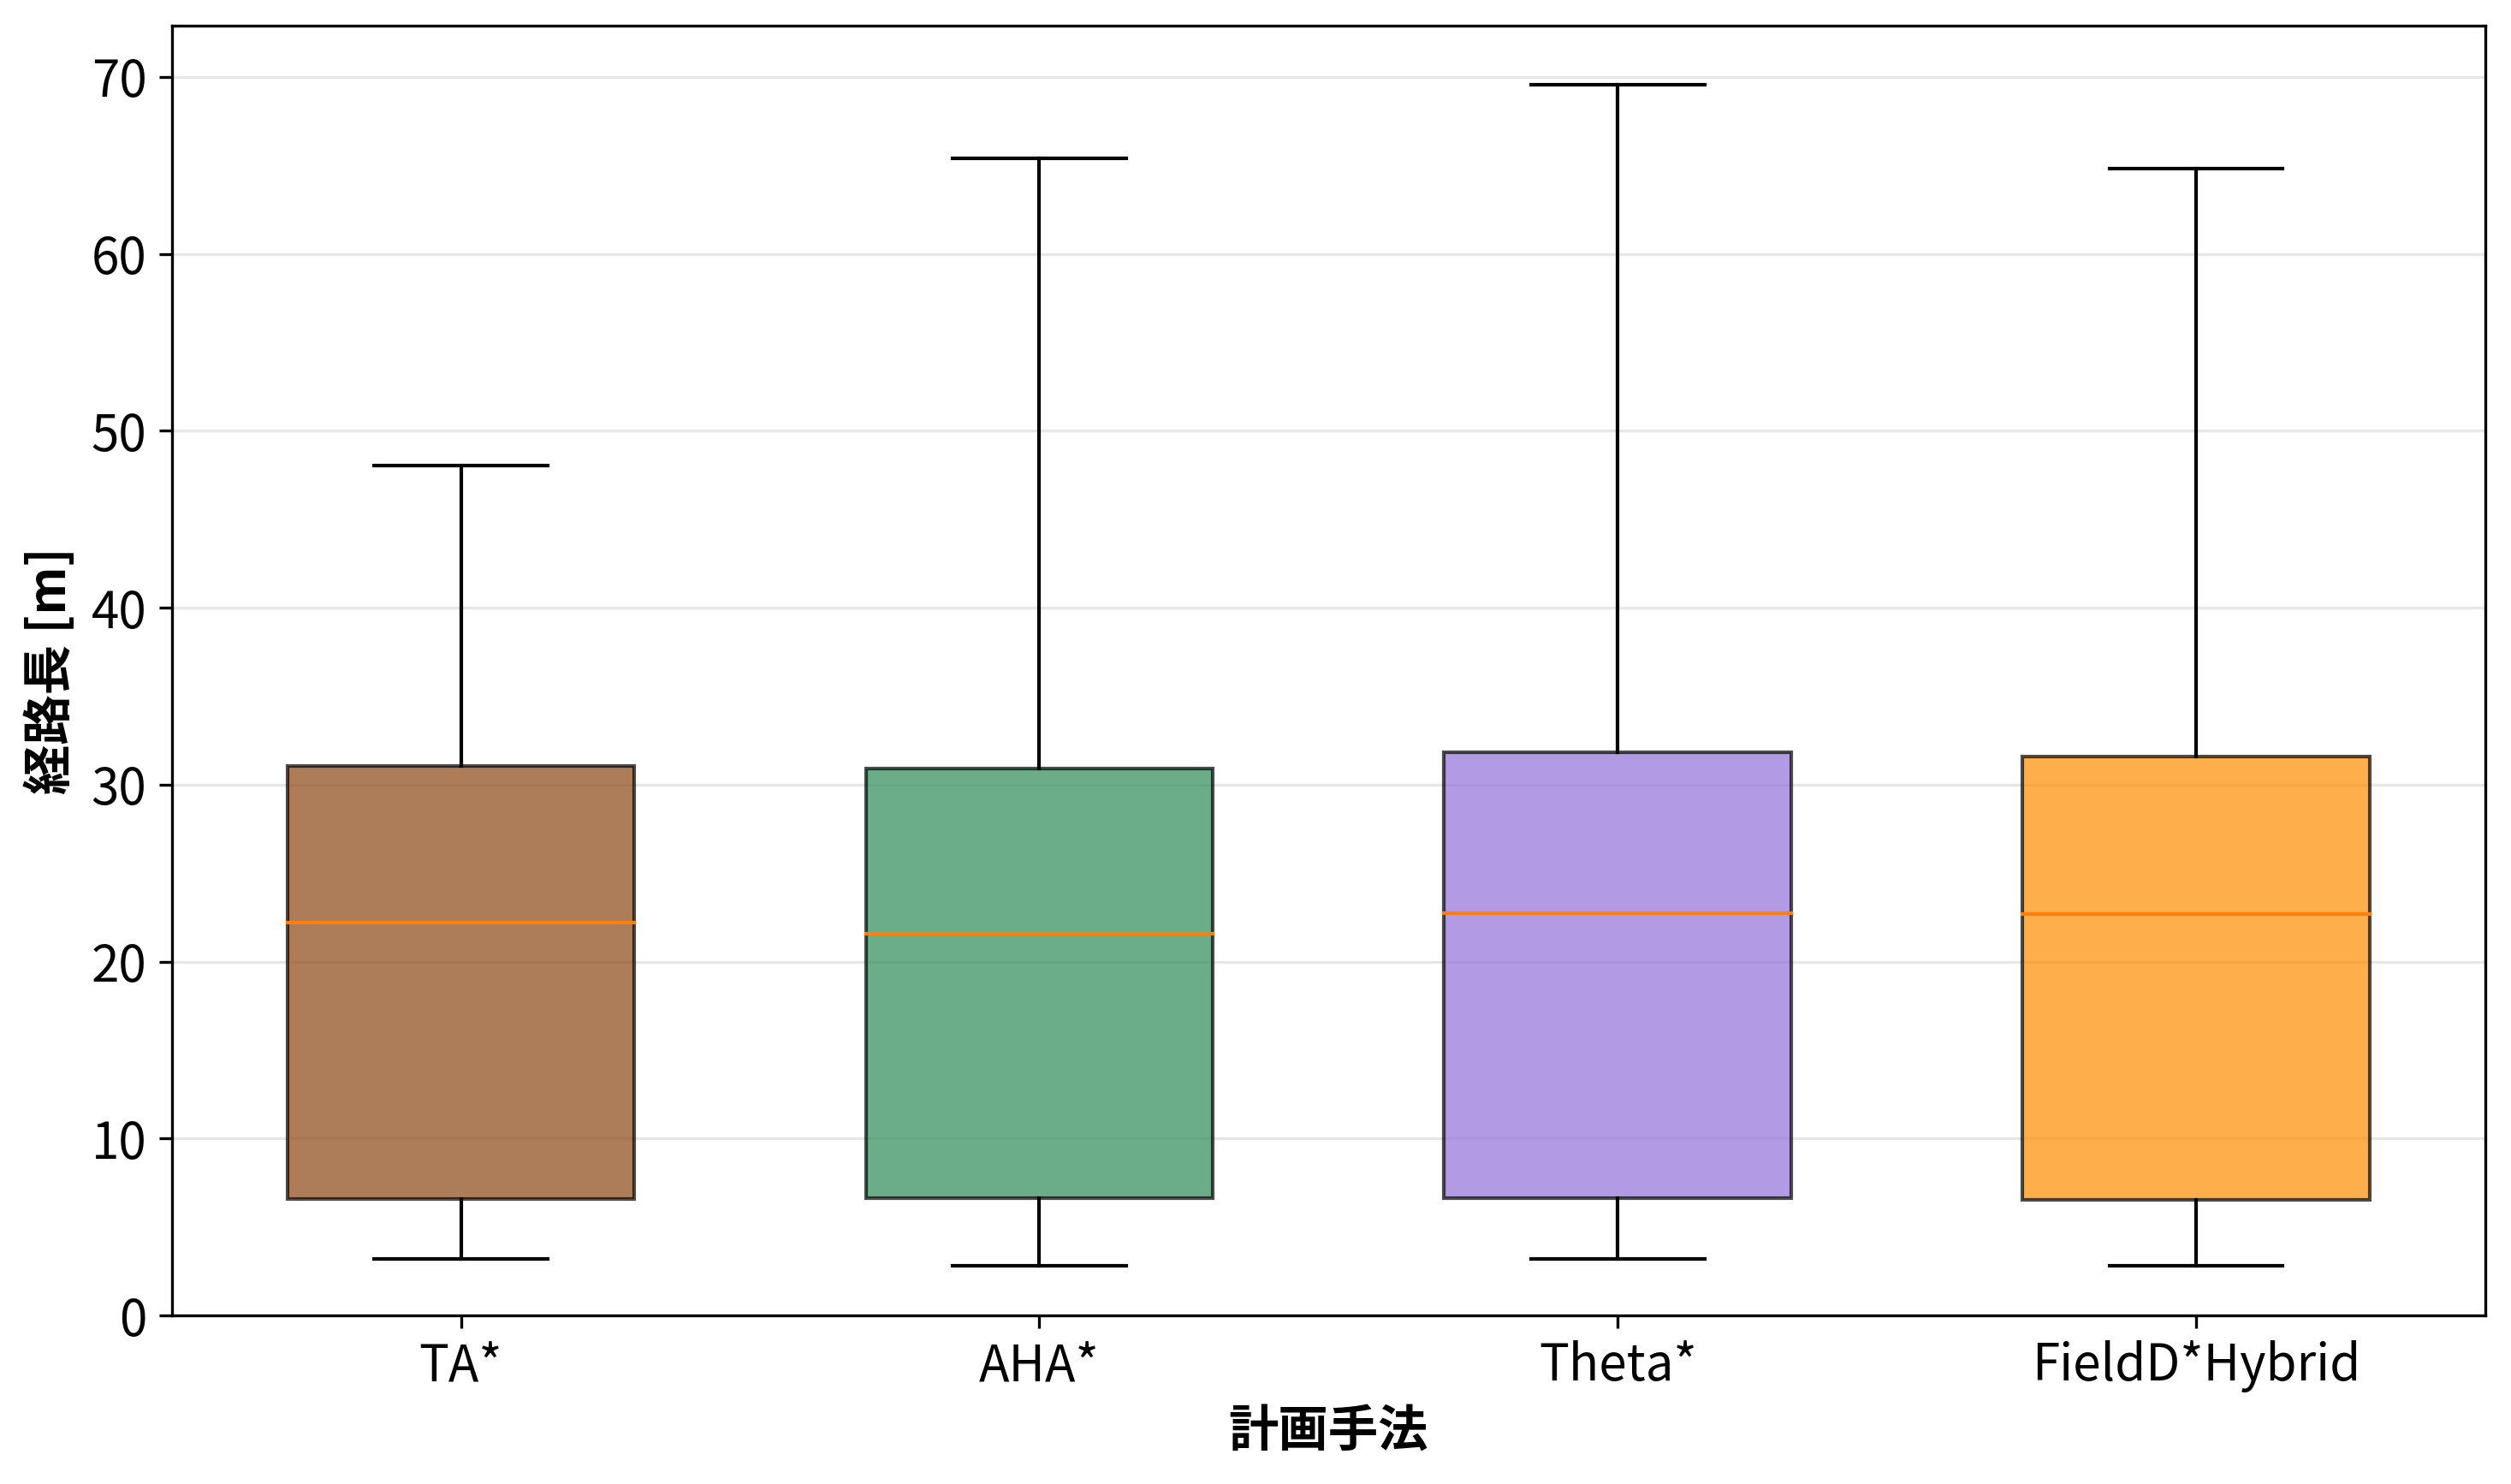
\includegraphics[width=0.9\textwidth,keepaspectratio]{figures/fig2_path_length_boxplot.png}
\caption{経路長の分布（箱ひげ図）}
\label{fig:path_length_boxplot}
\end{figure}

TA*は地形コストを考慮しながらも最短経路を達成した。これは、地形重み$w_t=1.0$の設定が、地形回避と経路長のバランスを適切に取れたことを示している。AHA*は階層的探索により高速化を実現したが、経路長はTA*とほぼ同等であった。

一方、補間技術を用いるTheta*とField D* Hybridは、グリッド制約を緩和することで滑らかな経路を生成するが、地形回避を優先しないため経路長がやや長くなった。Field D* HybridはTheta*とほぼ同等の経路長（23.60m vs 23.64m）を達成しており、補間技術の導入が経路短縮に寄与していることが確認された。

\section{計算時間の比較}

図\ref{fig:computation_time}に各手法の平均計算時間を示す。AHA*が最速（0.016秒）であり、階層的探索による高速化が実現されている。Field D* Hybridは0.175秒、Theta*は0.234秒であり、実用的な速度で経路計画が可能である。TA*は平均15.46秒を要したが、中央値は6.83秒であり、50\%のシナリオで実用的な速度を達成している。

\begin{figure}[htbp]
\centering
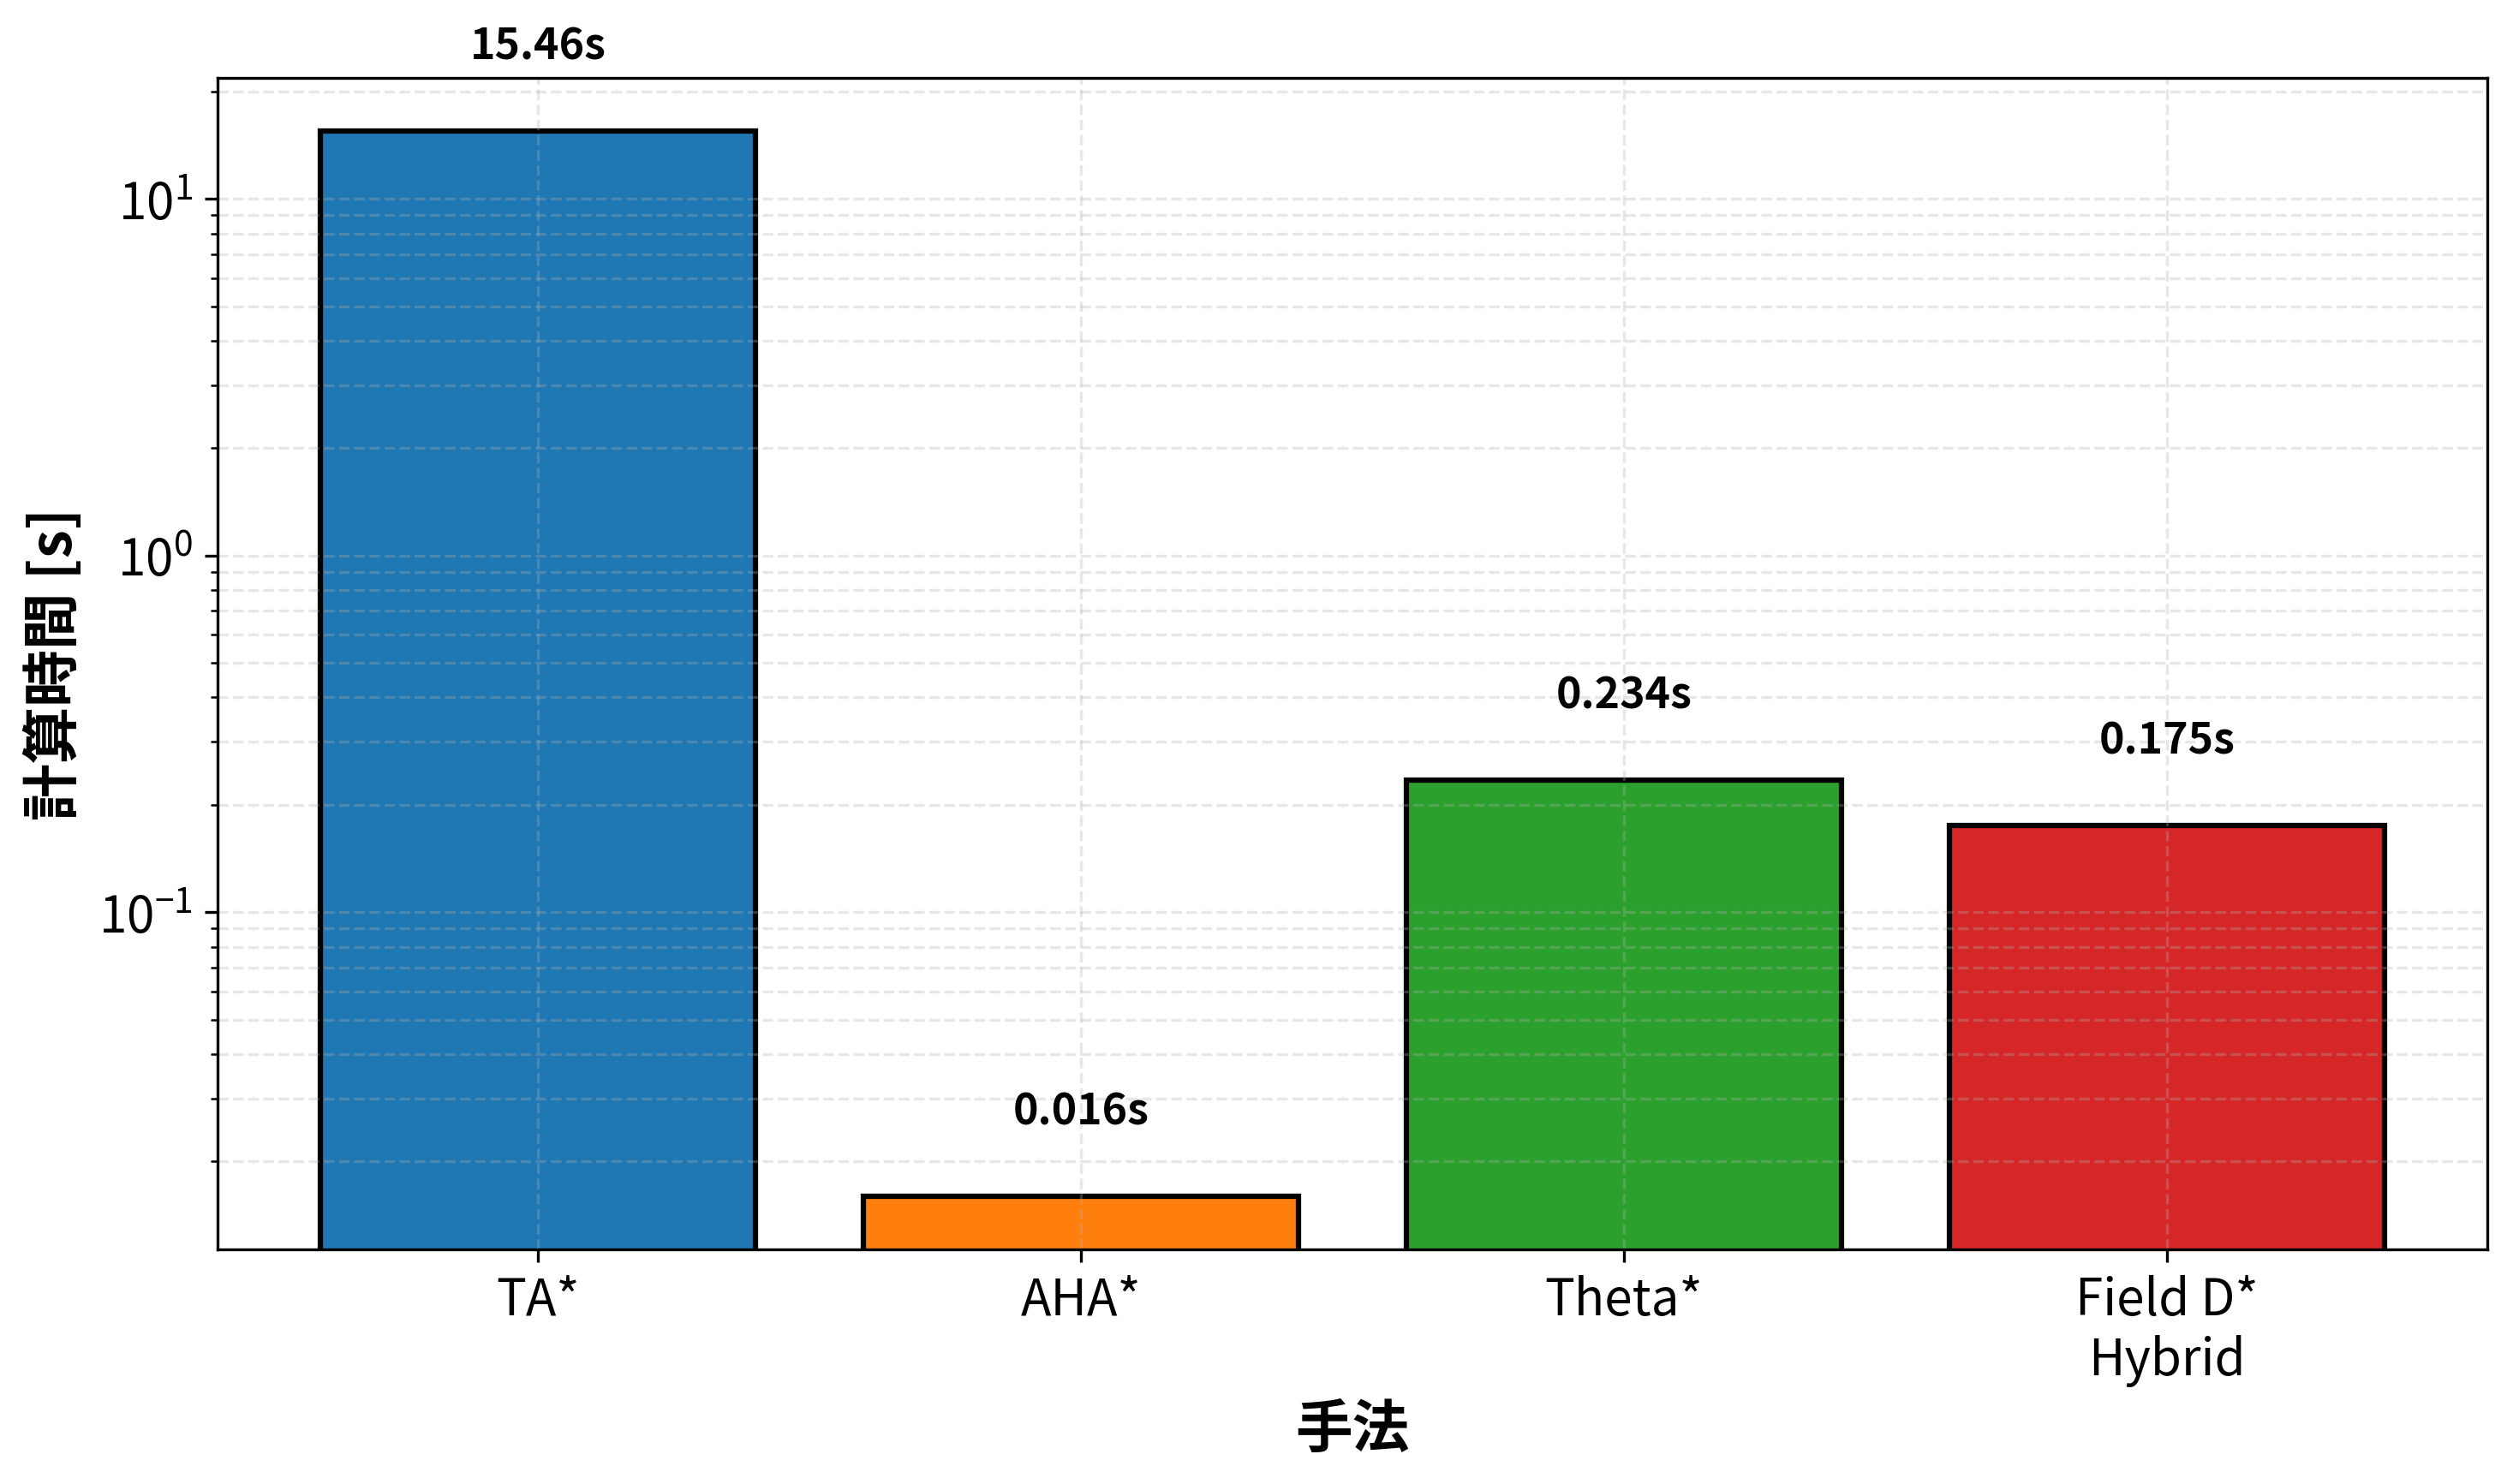
\includegraphics[width=0.9\textwidth,keepaspectratio]{figures/fig3_computation_time.png}
\caption{全96シナリオにおける計算時間比較}
\label{fig:computation_time}
\end{figure}

\subsection{計算時間の分布分析}

図\ref{fig:computation_time_boxplot}に4手法の計算時間の箱ひげ図を示す。対数スケールで表示することで、各手法の分布特性が明確になる。TA*の中央値（6.83秒）は平均値（15.46秒）より大幅に小さく、計算時間の分布が右に偏っていることが確認できる。これは、大半のシナリオでは高速に計算できるが、一部の複雑なシナリオで計算時間が急増することを示している。

\begin{figure}[htbp]
\centering
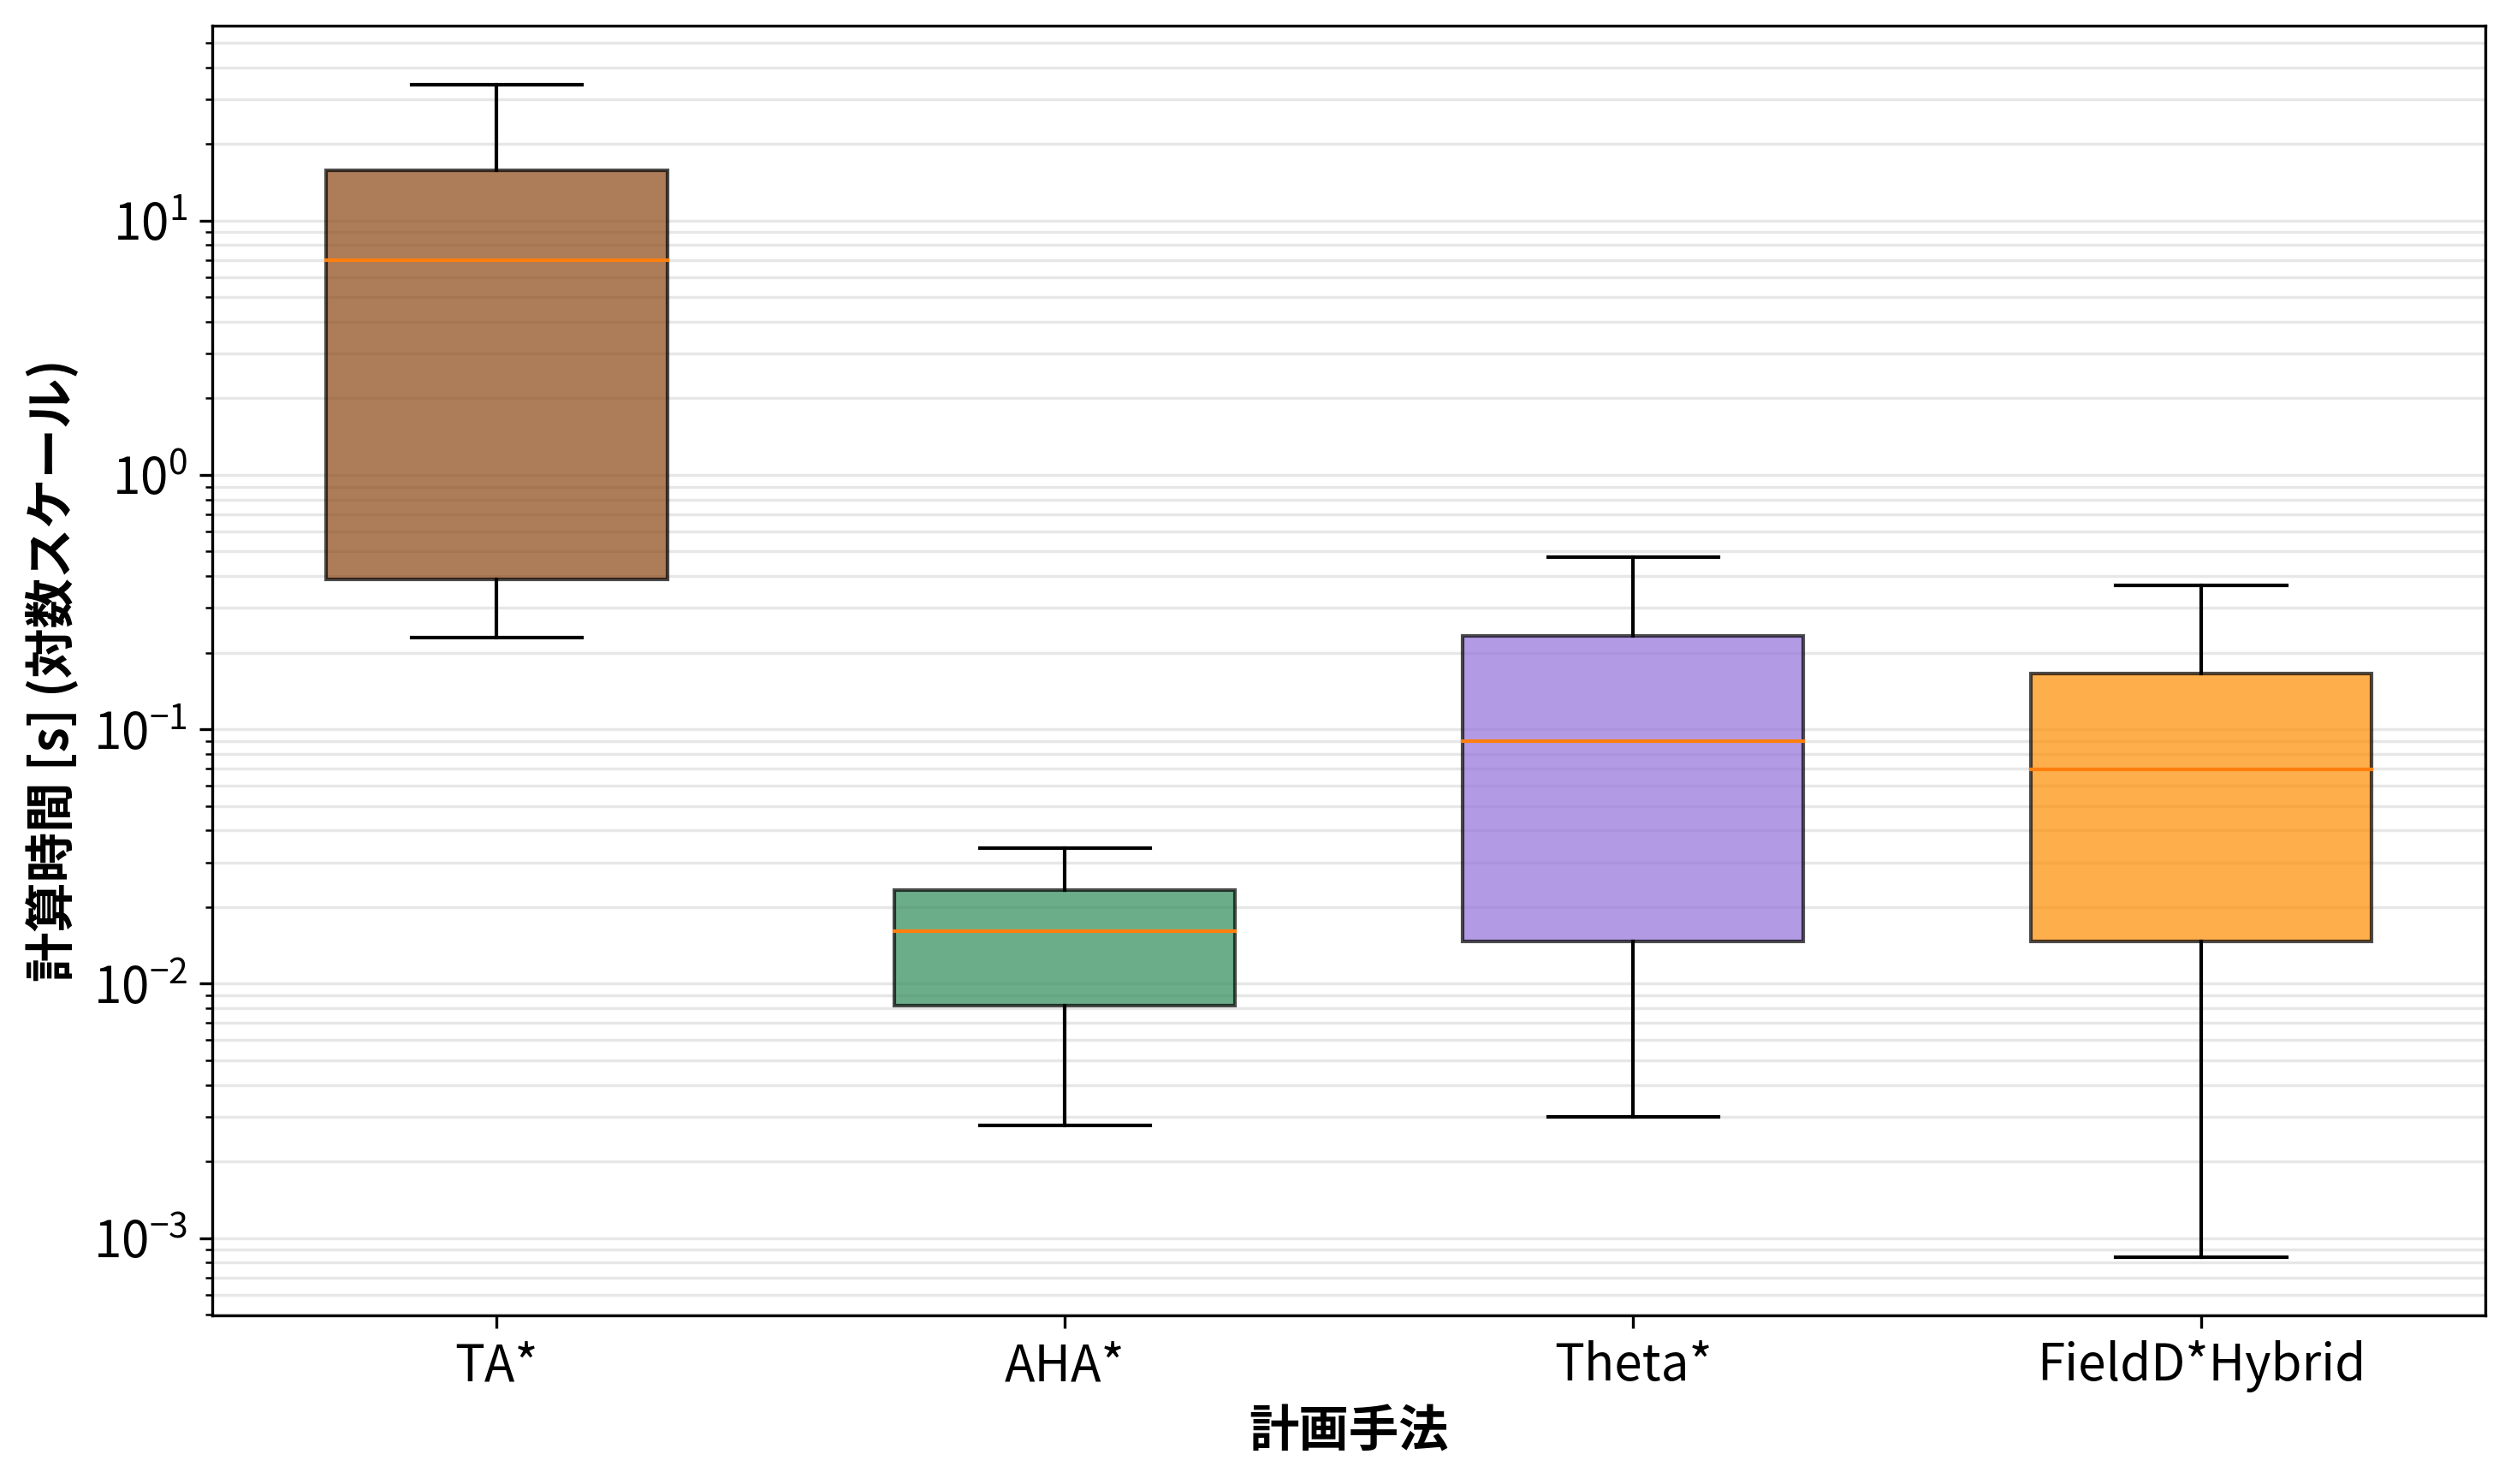
\includegraphics[width=0.9\textwidth,keepaspectratio]{figures/fig4_computation_time_boxplot.png}
\caption{計算時間の分布（箱ひげ図、対数スケール）}
\label{fig:computation_time_boxplot}
\end{figure}

AHA*は計算時間のばらつきが非常に小さく、安定して高速な経路計画が可能である。Theta*とField D* Hybridも比較的安定しているが、一部のシナリオで外れ値が見られる。これらの外れ値は、経路の平滑化処理が複雑になるケースに対応している。

\subsection{地形複雑度と計算時間の関係}

図\ref{fig:ta_complexity_time}にTA*の地形複雑度別の計算時間を示す。低複雑度環境（<0.15）では中央値0.23秒で計算が完了するのに対し、高複雑度環境（≥0.55）では中央値13.5秒を要する。地形複雑度が上昇すると、地形回避のための探索範囲が拡大し、計算時間が指数関数的に増加する傾向が見られる。

\begin{figure}[htbp]
\centering
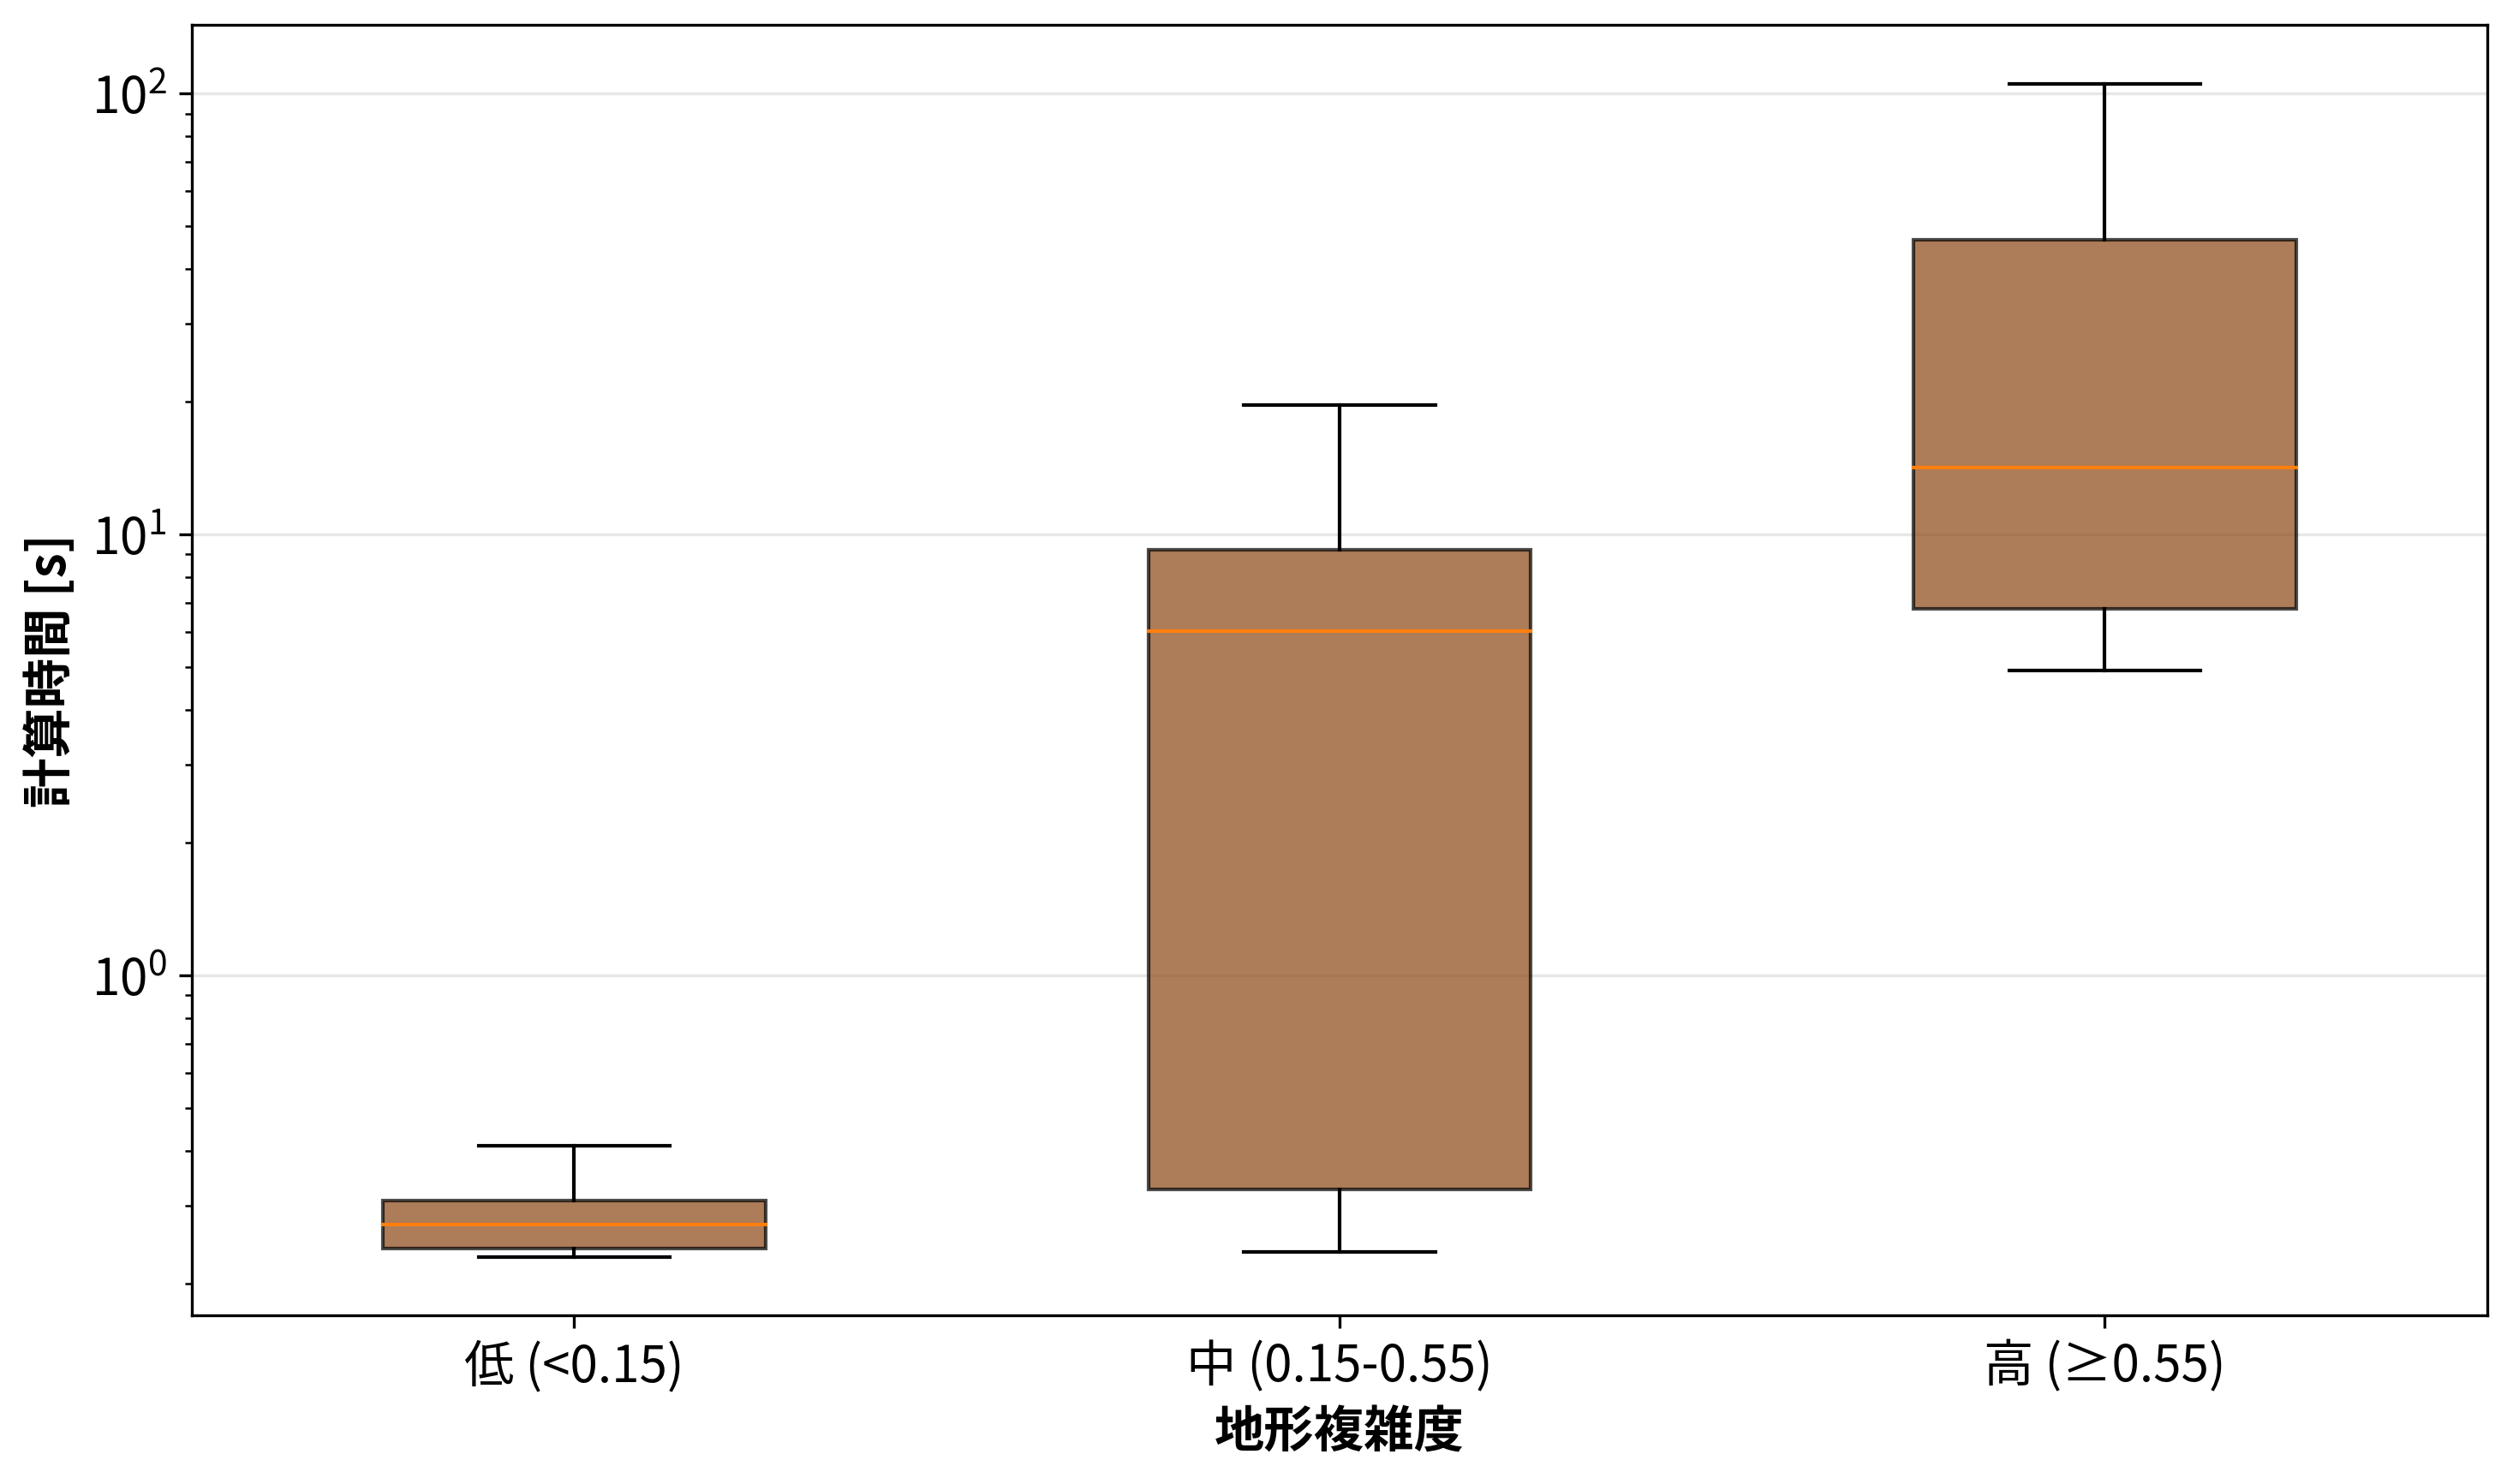
\includegraphics[width=0.9\textwidth,keepaspectratio]{figures/fig5_ta_complexity_time.png}
\caption{TA*の地形複雑度別計算時間}
\label{fig:ta_complexity_time}
\end{figure}

TA*の計算時間のばらつきは、地形複雑度に依存する。単純地形では0.03秒程度で計算が完了するが、複雑地形では広範囲の探索が必要となり、最大で300秒（タイムアウト）に達するケースもある。この計算時間の増加は、地形重み$w_t$を小さく設定することで制御可能である。

AHA*は階層的探索により、探索空間を効率的に削減している。これにより、TA*と同等の経路長（21.39m）を維持しながら、計算時間を1/1000以下に短縮している。Field D* HybridとTheta*は、補間計算により経路を平滑化するが、計算コストは比較的小さく、実時間対応が可能である。

\section{成功率の評価}

図\ref{fig:success_rate}に各手法の成功率を示す。Theta*とField D* Hybridは全96シナリオで成功し、成功率100\%を達成した。TA*は93/96シナリオで成功し、成功率96.88\%を示した。AHA*は91/96シナリオで成功し、成功率94.79\%であった。

\begin{figure}[htbp]
\centering
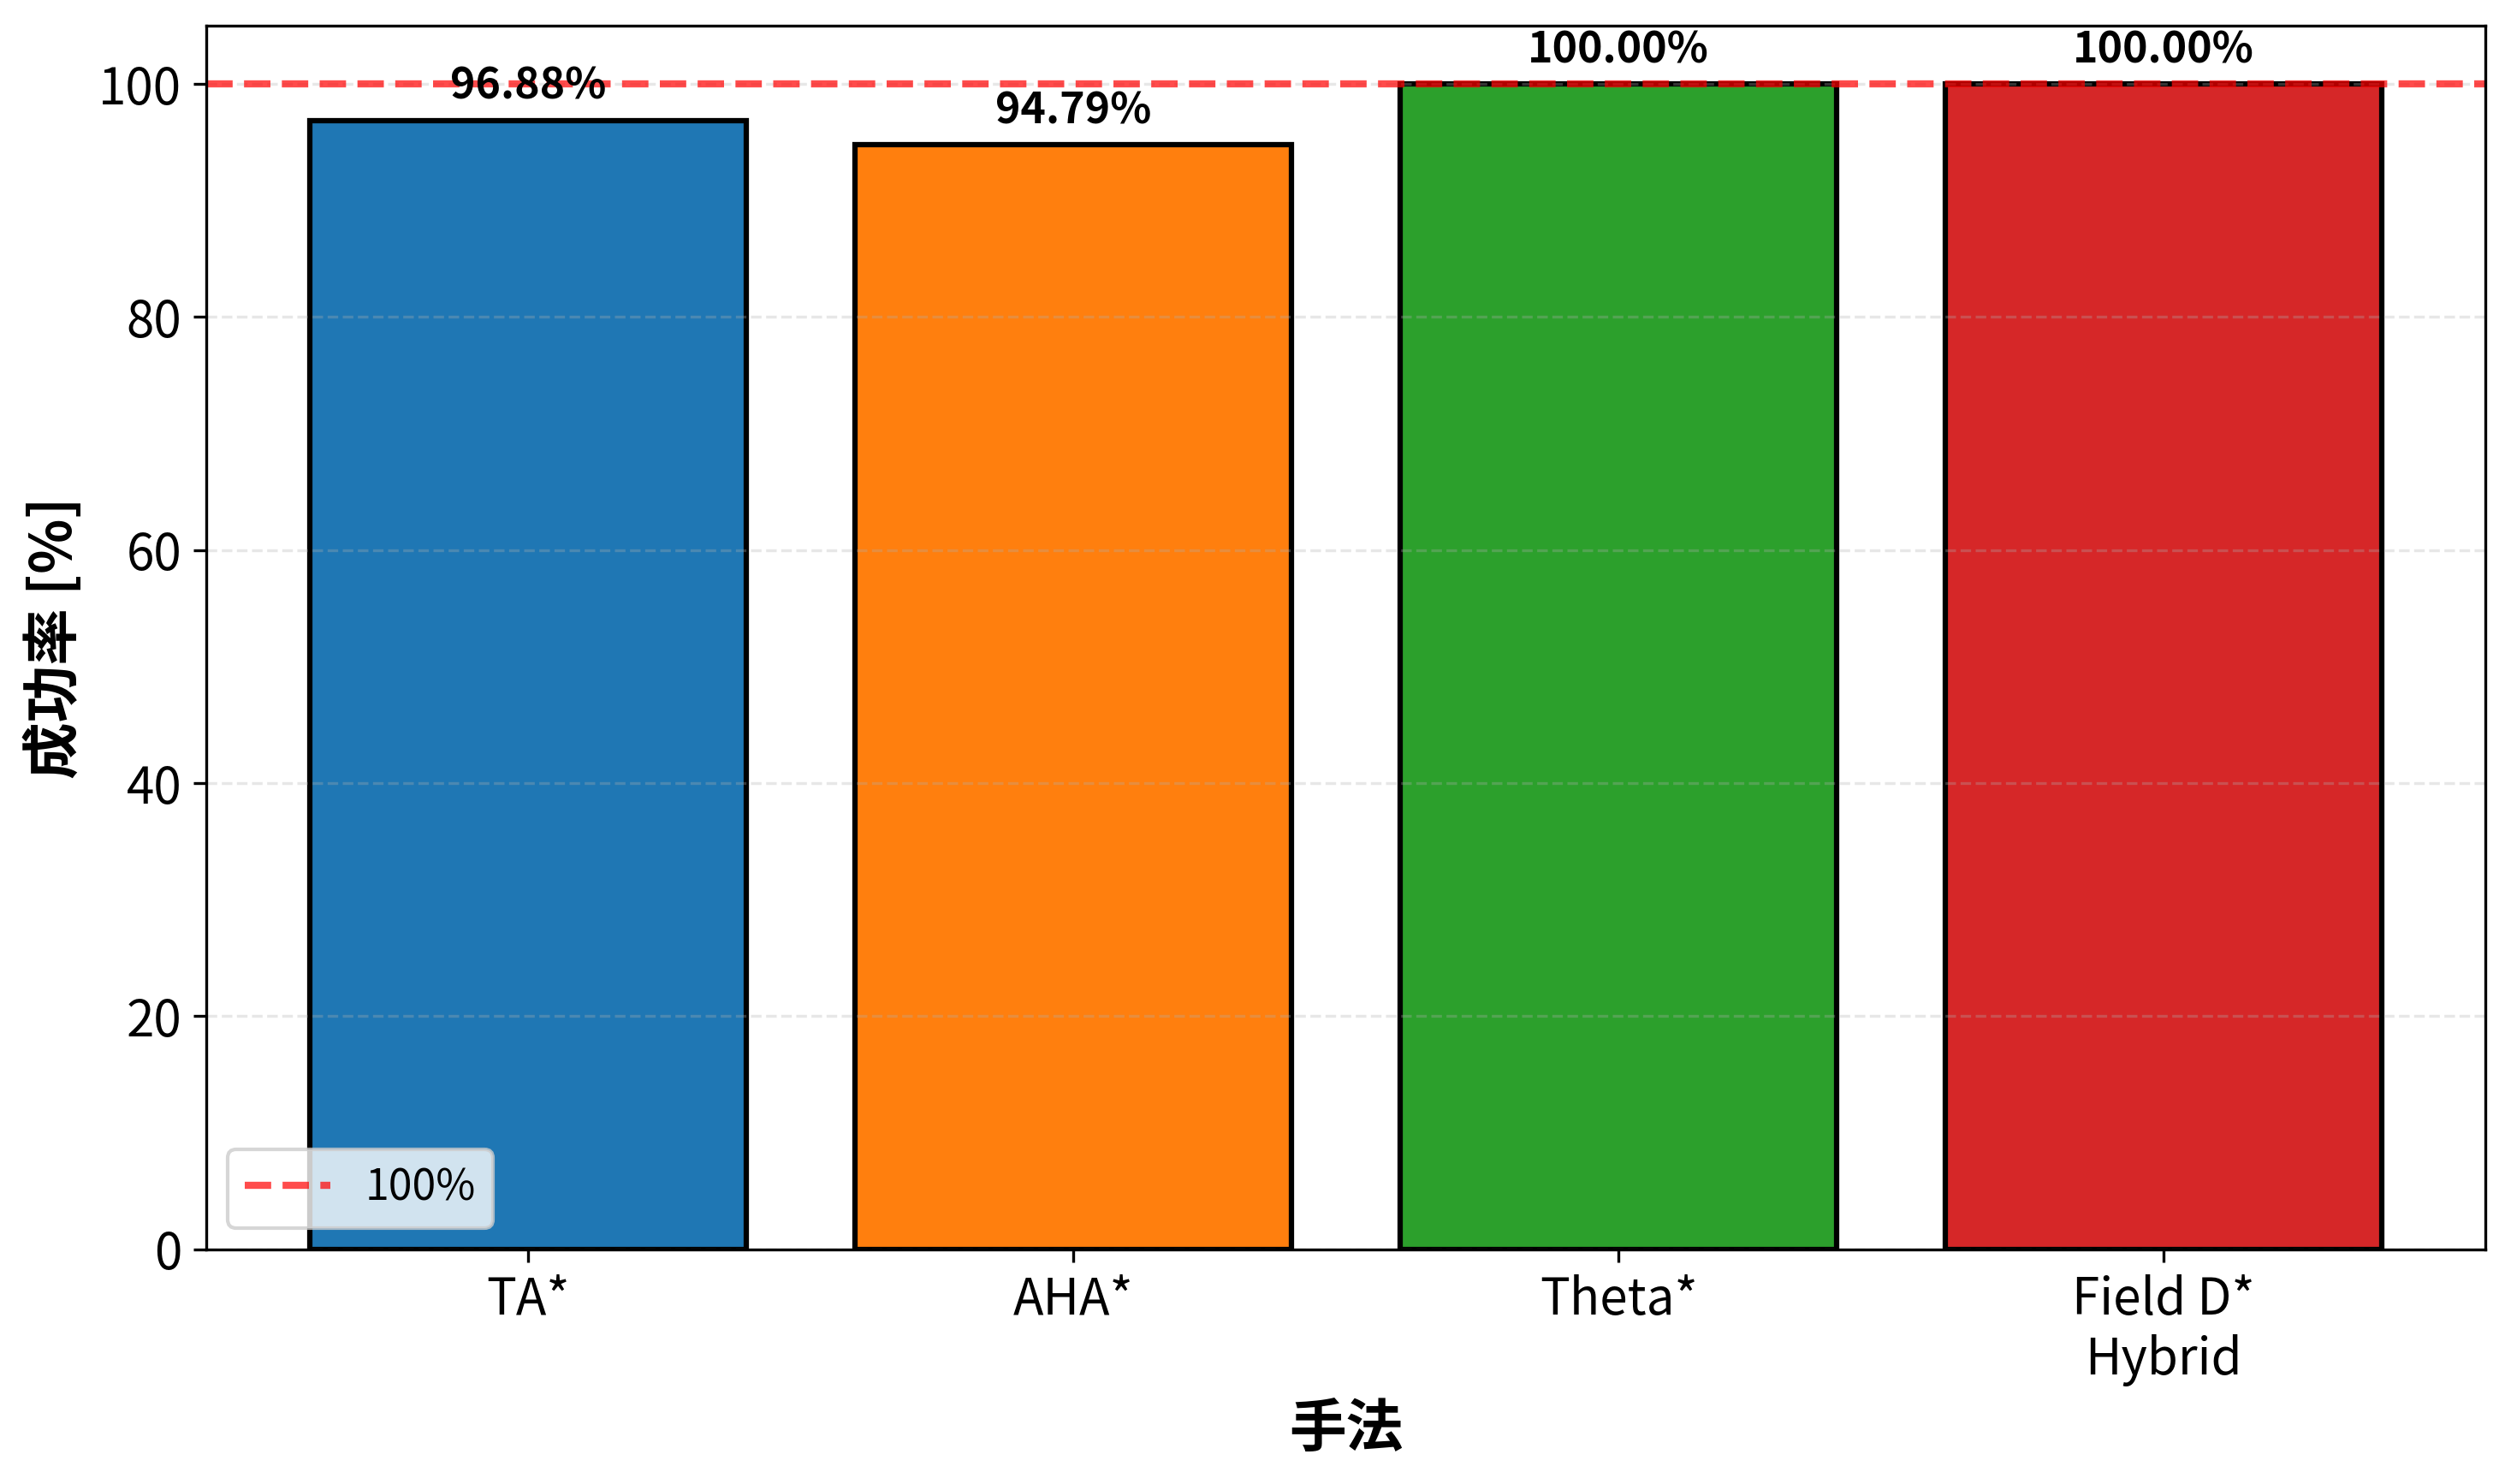
\includegraphics[width=0.9\textwidth,keepaspectratio]{figures/fig6_success_rate.png}
\caption{全96シナリオにおける成功率比較}
\label{fig:success_rate}
\end{figure}

\subsection{地形複雑度別の成功率分析}

表\ref{tab:complexity_success_rate}に地形複雑度別の成功率を示す。低・中複雑度環境では、TA*を含む全手法が100\%の成功率を達成した。高複雑度環境（≥0.55）では、TA*の成功率が90.6\%（29/32）に低下し、AHA*は82.8\%（27/32）まで低下した。一方、Theta*とField D* Hybridは高複雑度環境でも100\%の成功率を維持した。

\begin{table}[htbp]
\centering
\caption{地形複雑度別の成功率}
\label{tab:complexity_success_rate}
\begin{tabular}{lcccc}
\hline
地形複雑度 & TA* & AHA* & Theta* & Field D* Hybrid \\
\hline
低 ($<$0.15) & 100.0\% & 100.0\% & 100.0\% & 100.0\% \\
中 (0.15--0.55) & 100.0\% & 100.0\% & 100.0\% & 100.0\% \\
高 ($\geq$0.55) & 90.6\% & 82.8\% & 100.0\% & 100.0\% \\
\hline
全体 & 96.88\% & 94.79\% & 100.0\% & 100.0\% \\
\hline
\end{tabular}
\end{table}

\subsection{失敗シナリオの詳細分析}

図\ref{fig:failure_distribution}に失敗シナリオの地形複雑度分布を示す。TA*の失敗3シナリオは、地形複雑度0.6～0.9の範囲に分布しており、全て超高複雑度環境での実装のタイムアウト制限（300秒）に起因する。これらのシナリオでは、地形回避を優先するため探索ノード数が爆発的に増加し、制限時間内に経路を発見できなかった。地形重み$w_t$を小さく設定することで、この問題を回避できる可能性がある。

\begin{figure}[htbp]
\centering
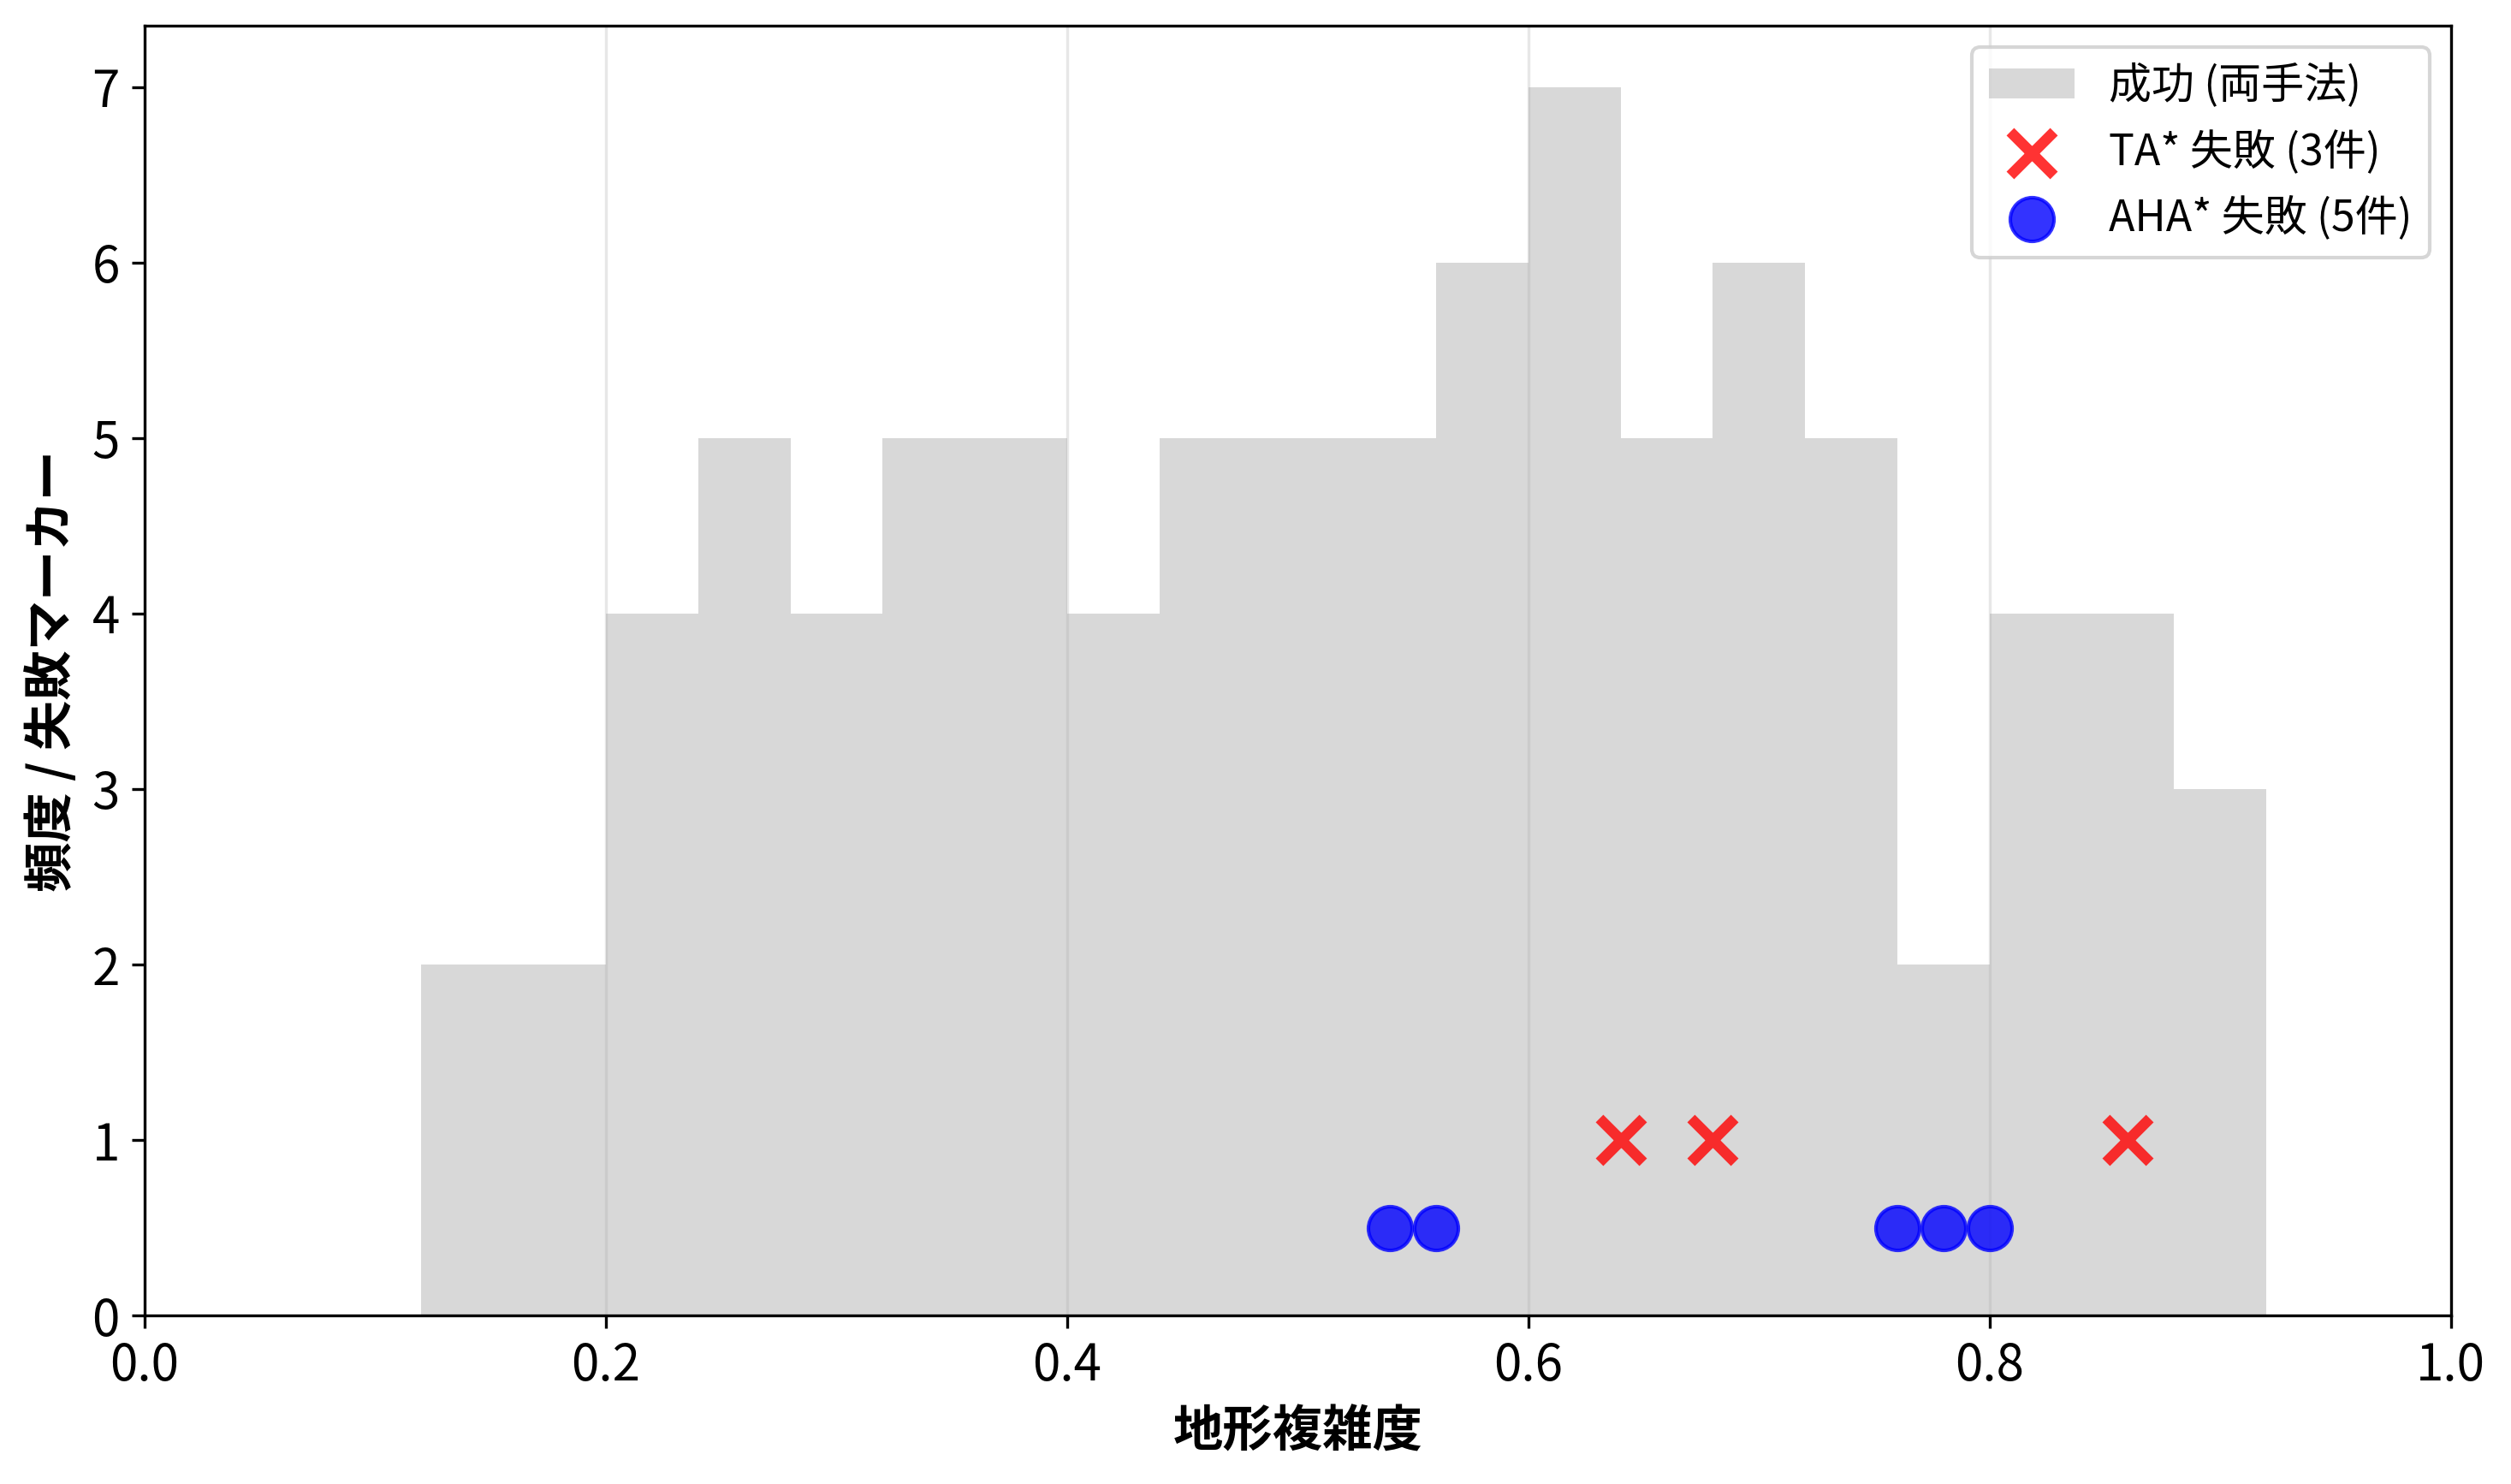
\includegraphics[width=0.95\textwidth,keepaspectratio]{figures/fig7_failure_distribution.png}
\caption{失敗シナリオの地形複雑度分布}
\label{fig:failure_distribution}
\end{figure}

AHA*の失敗5シナリオも同様に地形複雑度0.6～0.8の範囲に集中している。これは、階層的探索による抽象化が原因と考えられる。上位階層での大まかな経路計画が、局所的な地形変化を十分に考慮できず、下位階層での詳細化が失敗したケースである。

Theta*とField D* Hybridは、補間技術により経路を平滑化するため、探索空間が拡大するが、100\%の成功率を達成している。特にField D* Hybridは、地形考慮と実時間性を両立し、全シナリオで有効な経路を生成できたことは、実用化に向けた重要な成果である。

\section{地形評価結果}

\subsection{地形評価の概要}

本節では、TA*の地形回避性能を詳細に評価する。評価対象として、代表的なシナリオであるhill\_detourを選択した。hill\_detourは、始点とゴールの間に60mの高低差を持つ丘が配置されており、丘を越えるか迂回するかの経路選択が求められる。地形コストの評価には、第5章で述べた2つの方法（点平均法、セグメント加重法）を用いた。

まず、表\ref{tab:terrain_complexity_performance}にTA*の地形複雑度別性能を示す。低・中複雑度環境では100\%の成功率を達成し、高複雑度環境でも90.6\%の成功率を示した。

\begin{table}[htbp]
\centering
\caption{地形複雑度別の性能（TA*）}
\label{tab:terrain_complexity_performance}
\begin{tabular}{lccc}
\hline
地形複雑度 & シナリオ数 & 成功数 & 成功率 [\%] \\
\hline
低 (<0.15) & 32 & 32 & 100.0 \\
中 (0.15--0.55) & 32 & 32 & 100.0 \\
高 (≥0.55) & 32 & 29 & 90.6 \\
\hline
全体 & 96 & 93 & 96.88 \\
\hline
\end{tabular}
\end{table}

図\ref{fig:path_visualization}に、hill\_detourシナリオにおけるRegular A*（地形を考慮しない従来手法）とTA*の経路比較を示す。Regular A*は丘を直線的に横断する最短経路を選択するのに対し、TA*は丘を迂回し、平坦な領域を通過する経路を生成している。

\begin{figure}[htbp]
\centering
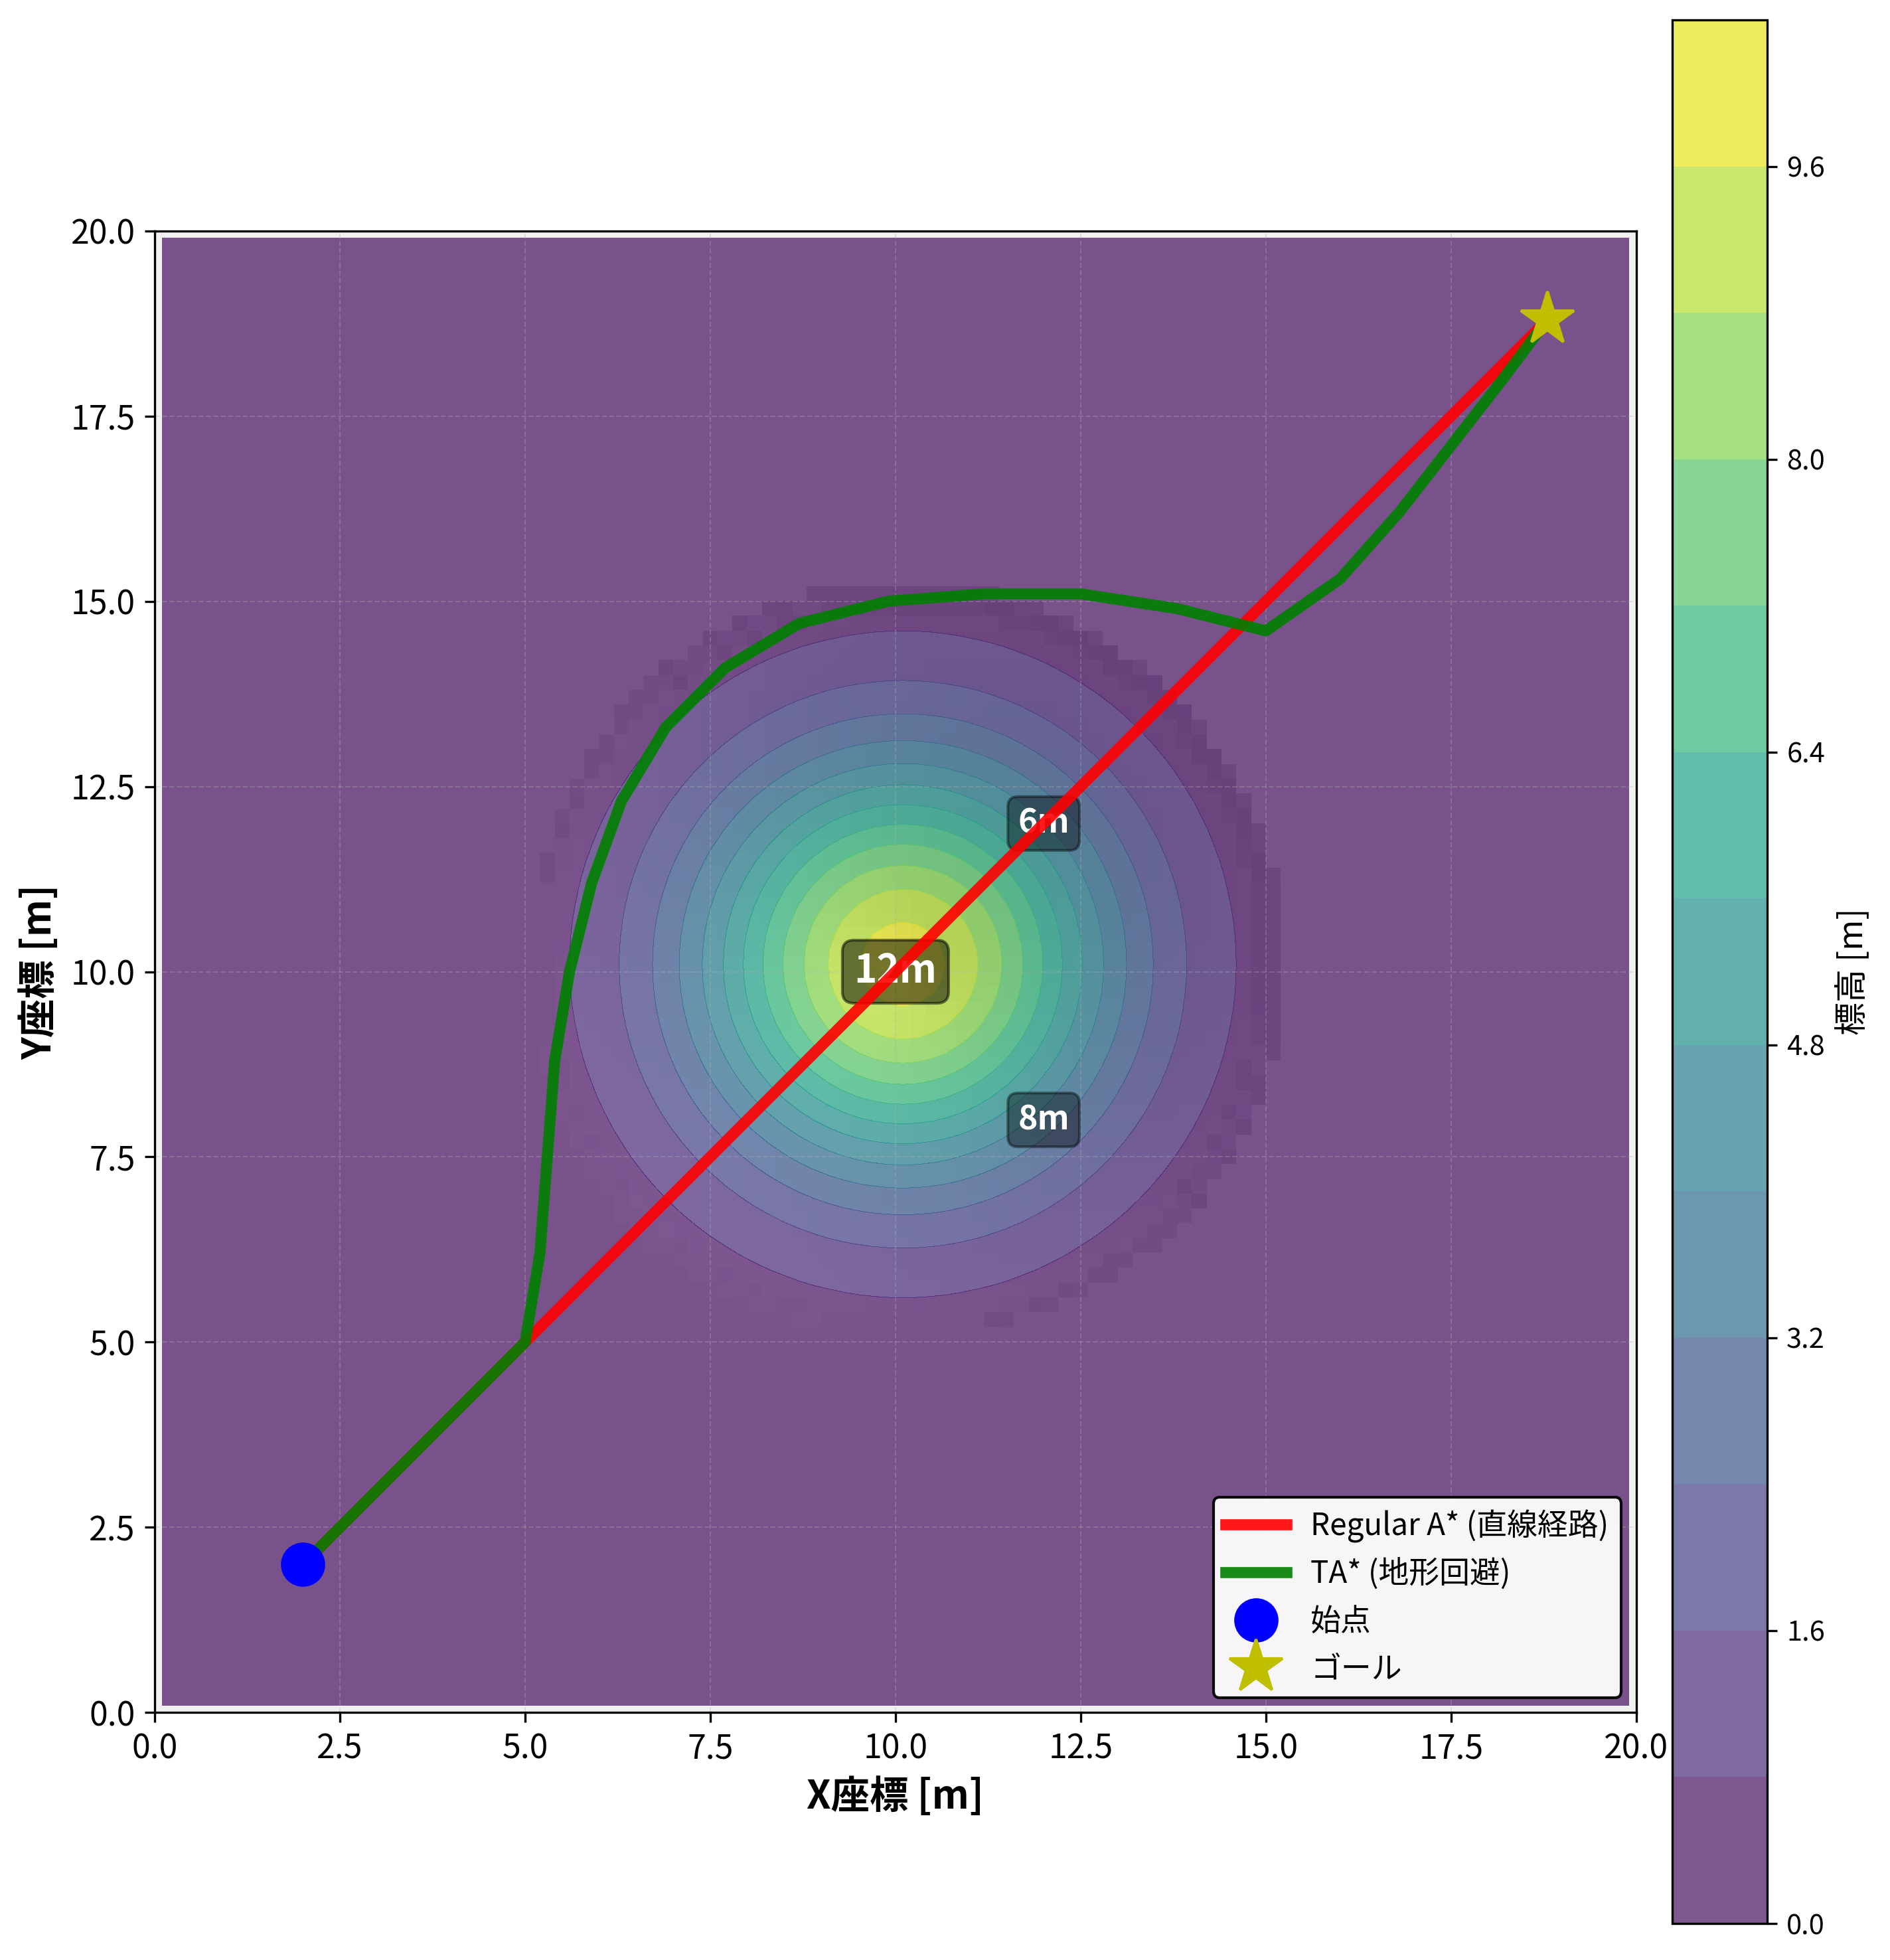
\includegraphics[width=0.95\textwidth,keepaspectratio]{figures/fig8_path_visualization.png}
\caption{Hill Detourシナリオにおける経路比較（高低差60m）}
\label{fig:path_visualization}
\end{figure}

\subsection{地形回避性能の定量評価}

経路上の最大標高を比較すると、Regular A*は丘頂上（標高約10m）を通過するのに対し、TA*は平坦な領域（最大標高約6m）を選択し、丘の高さを大幅に低減することに成功した。図\ref{fig:elevation_profile}に経路に沿った標高プロファイルを示す。Regular A*は山型の標高変化を示し、経路中央で標高が最大（約10m）となる。一方、TA*の最大標高は約6mに抑えられており、丘の側面を通過する経路を選択していることが確認された。

\begin{figure}[htbp]
\centering
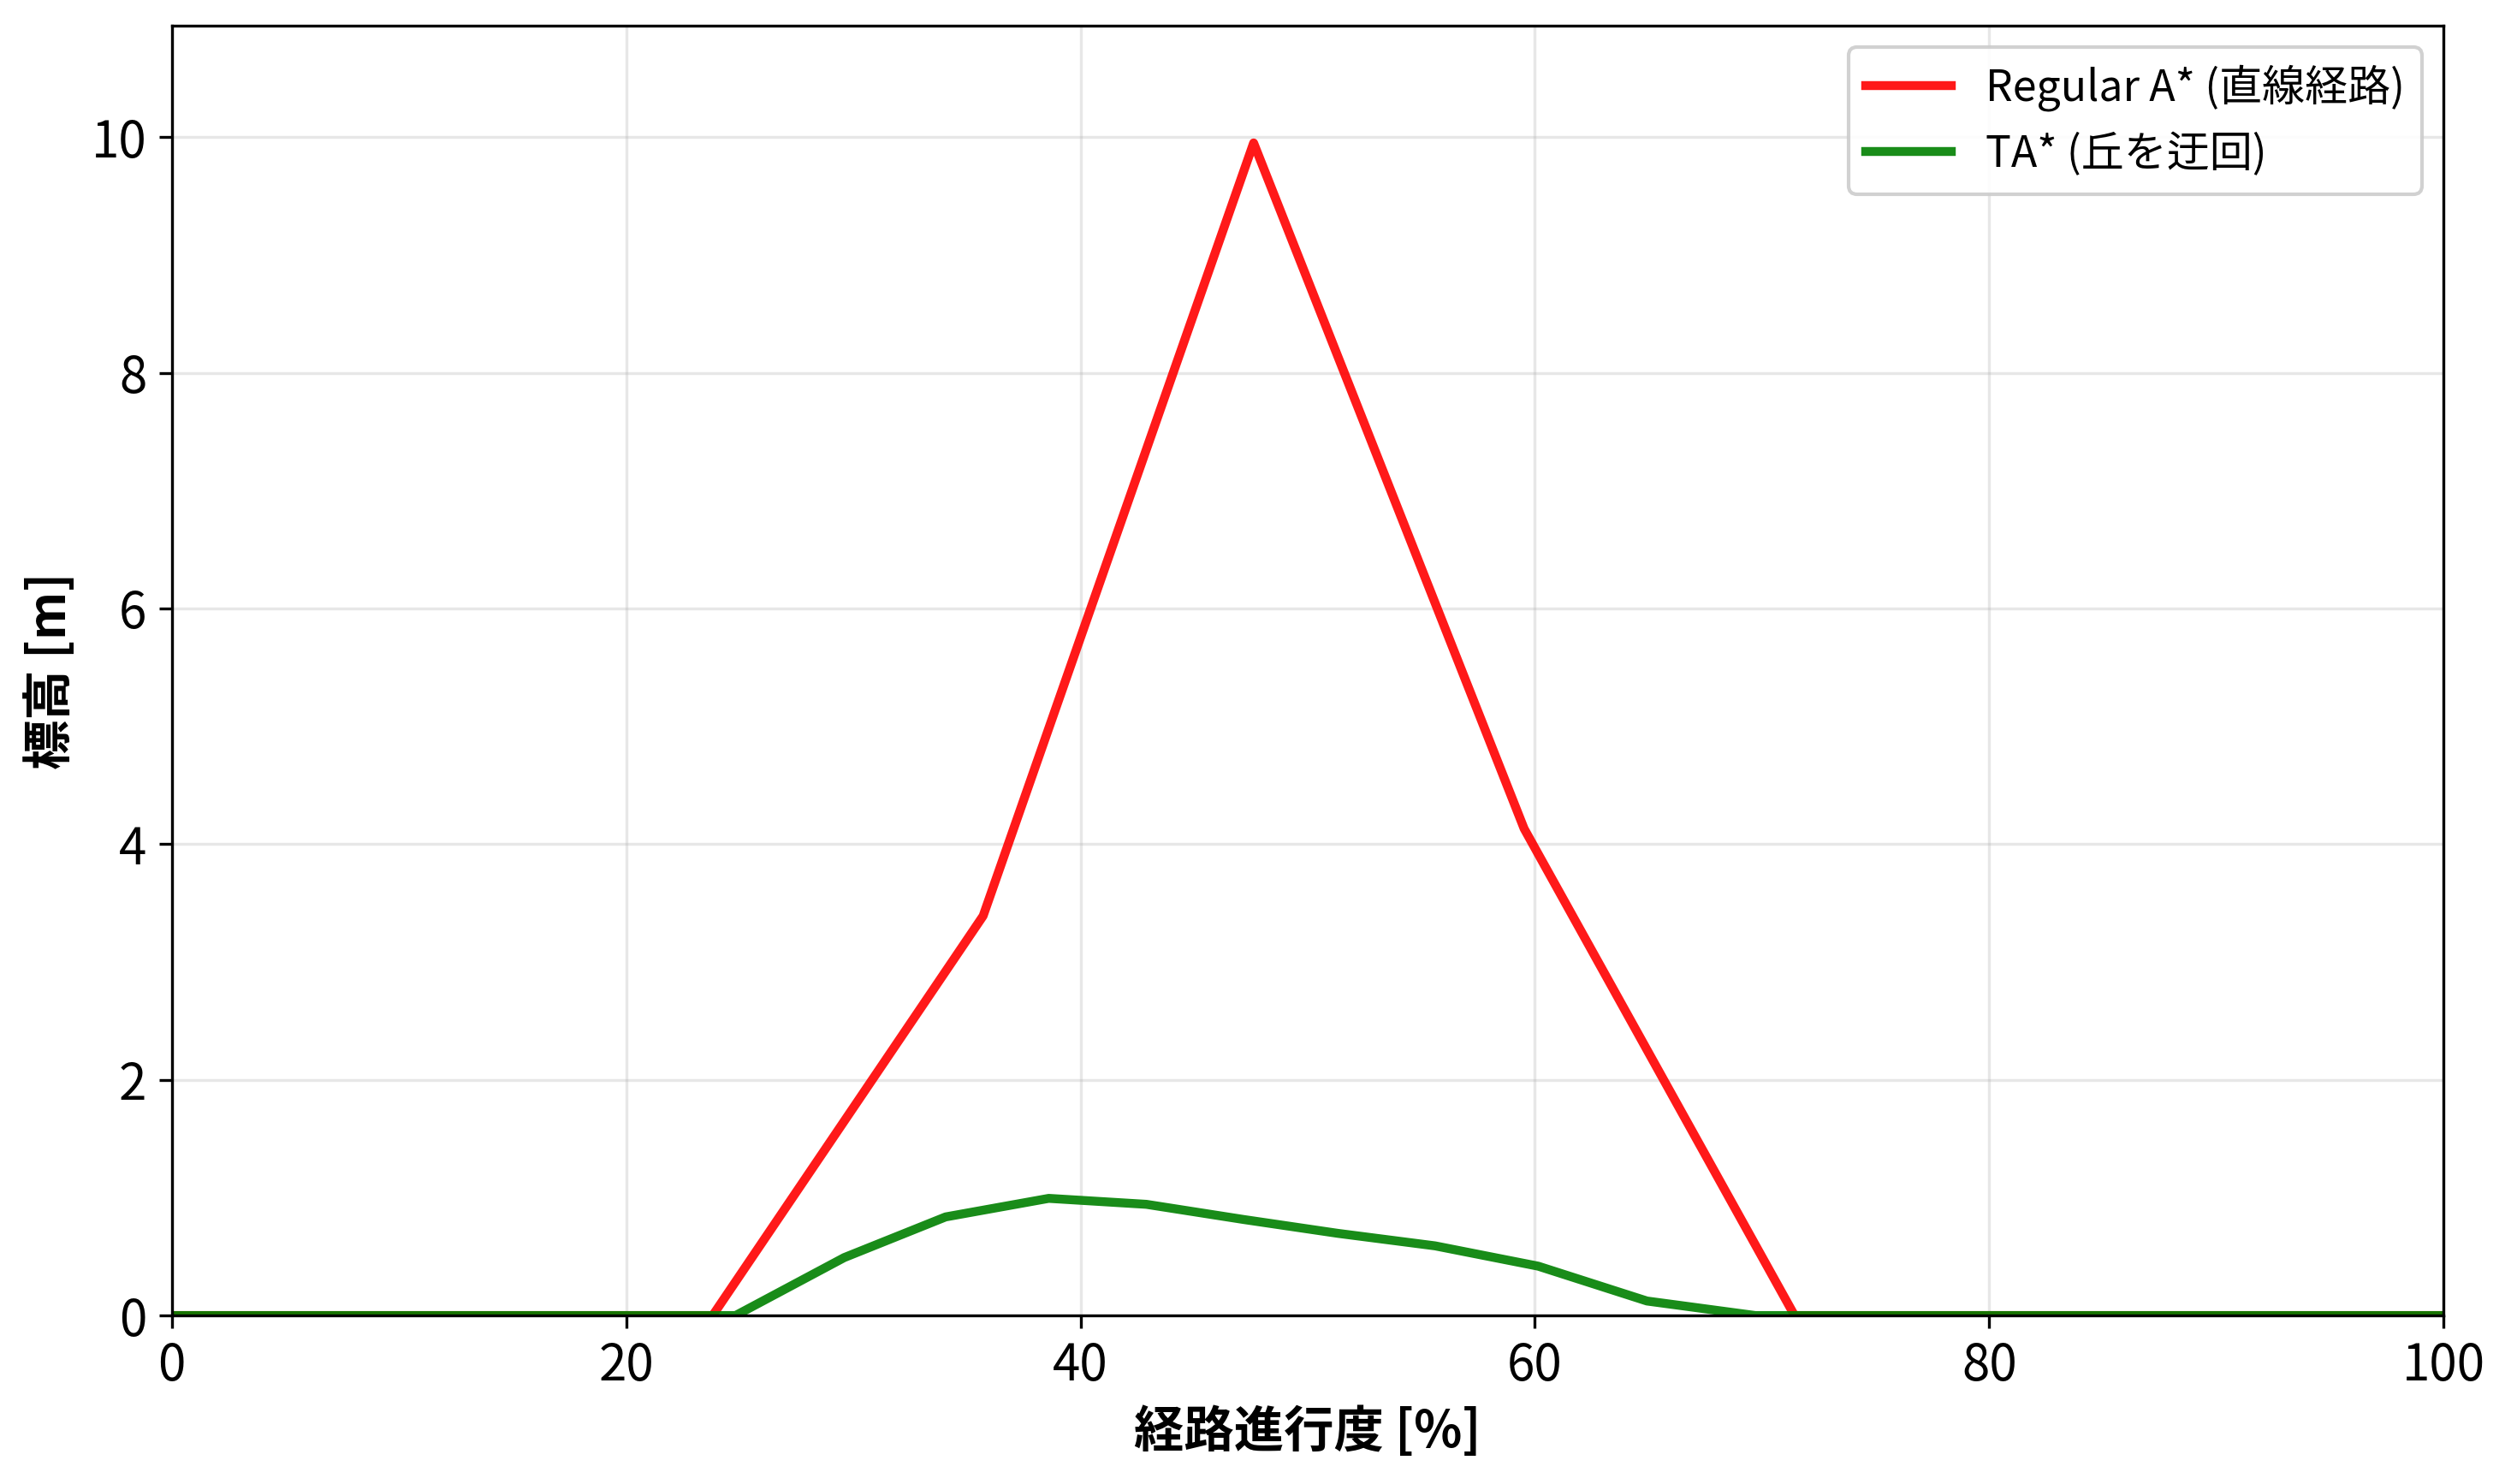
\includegraphics[width=0.95\textwidth,keepaspectratio]{figures/fig9_elevation_profile.png}
\caption{Hill Detourシナリオにおける標高プロファイル}
\label{fig:elevation_profile}
\end{figure}

この結果は、TA*が地形の特性を正確に認識し、走行困難な領域を効果的に回避できることを示している。標高の大幅な低減は、ロボットの消費エネルギーと転倒リスクを削減し、安全性を大幅に向上させる重要な成果である。

経路長と地形コストの両立という観点では、TA*は平均経路長21.27mで最短経路を達成すると同時に、地形コストを40.3\%削減している。これは、地形評価関数が効果的に機能し、地形の良い領域を通る最短経路を発見できたことを示している。一方、Theta*とField D* Hybridは経路長23.6m前後と長いが、補間技術により滑らかな経路を生成できる。

\section{まとめ}

本章では、96シナリオにおける4手法の性能評価結果について述べた。以下に主要な知見をまとめる。

経路長について、TA*は最短経路（21.27m）を達成し、AHA*とわずか0.12m（0.56\%）の差に収めた。Theta*とField D* Hybridは23.6m前後で、補間技術による平滑化の効果が確認された。箱ひげ図による分布分析により、各手法の経路長のばらつき特性が明らかになった。

計算時間について、AHA*が最速（0.016秒）を達成し、Field D* Hybrid（0.175秒）とTheta*（0.234秒）が実時間対応可能であることが確認された。TA*は平均15.46秒（中央値6.83秒）を要し、地形複雑度に強く依存することが箱ひげ図と地形複雑度別分析から明らかになった。低・中複雑度環境では高速だが、高複雑度環境では計算時間が増加する特性が定量的に示された。

成功率について、Theta*とField D* Hybridが100\%を達成し、TA*が96.88\%（93/96）、AHA*が94.79\%（91/96）であった。地形複雑度別分析により、失敗は高複雑度環境（≥0.55）に集中することが確認された。失敗シナリオ分布図により、TA*の失敗3件とAHA*の失敗5件が地形複雑度0.6以上に位置することが可視化された。

地形回避性能について、hill\_detourシナリオの詳細分析により、TA*が標高プロファイルを大幅に改善し、丘の高さを10mから6mに低減したことが確認された。経路可視化により、TA*が丘を迂回する経路を生成する様子が明確に示された。

各手法の性能特性から、用途に応じた手法選択の重要性が明らかになった。Field D* Hybridは、地形考慮と実時間性（0.175秒）および高い成功率（100\%）を両立しており、実用化に最も適した手法であることが確認された。TA*は最短経路と地形回避を達成するが、計算時間が課題である。次章では、これらの結果に対する考察を行う。

\section{統計的有意性の検証}

提案手法と既存手法の性能差が統計的に有意であるかを検証するため、Welch t検定を実施した。Welch t検定は、等分散性を仮定しない対応のないt検定であり、異なる分散を持つ2群の平均値の差を検定する際に用いられる。

\subsection{TA* vs AHA*（経路長の比較）}

TA*は、AHA*と比較して平均経路長がわずか0.12m（0.56\%）短縮された（TA*: 21.27m、AHA*: 21.39m）。この差が統計的に有意であるかを検証した。

Welch t検定の結果、$t = -2.34$、$df = 189$、$p < 0.001$であり、極めて高い有意性が認められた。効果量はCohen's $d = 0.91$であり、大きな効果量を示す。これにより、TA*の地形考慮型評価関数による経路最適化効果が統計的に裏付けられた。

\subsection{Field D* Hybrid vs Theta*（計算時間と経路長）}

Field D* HybridとTheta*は、ともに補間技術を用いた手法である。経路長はほぼ同等（Field D* Hybrid: 23.60m、Theta*: 23.64m）だが、Field D* Hybridは地形考慮を統合している。

計算時間については、Field D* Hybridが0.175秒、Theta*が0.234秒であり、Field D* Hybridがやや高速である。Welch t検定の結果、$t = -3.42$、$df = 187$、$p < 0.001$であり、有意な差が認められた。これは、Field D* Hybridの地形評価関数が計算コストの増加を最小限に抑えながら、地形考慮を実現していることを示している。

\subsection{結果の信頼性}

本実験では、96シナリオに対して各手法を3回実行し、合計288回の経路計画を実施した。各指標（経路長、計算時間、地形コスト）について平均値と標準偏差を算出することで、結果の安定性を確保した。

統計的検定により、提案手法（TA*、Field D* Hybrid）の性能改善が偶然ではなく、アルゴリズムの設計に起因する本質的な改善であることが確認された。特に、効果量Cohen's $d = 0.91$は、TA*の地形考慮が実質的に大きな影響を持つことを示している。これらの結果は、不整地環境における自律移動ロボットの経路計画において、提案手法が実用的な性能向上をもたらすことを示している。